% The ICIP2016 paper according to the given template
%          spconf.sty  - ICASSP/ICIP LaTeX style file, and
%          IEEEbib.bst - IEEE bibliography style file.
% --------------------------------------------------------------------------
\documentclass{article}
\usepackage{spconf,amsmath,graphicx}
\usepackage{enumitem}
\usepackage{verbatim}

% Definitions.
% --------------------
\def\B{{\mathbf B}}
\def\M{{\mathbf M}}
\def\I{{\mathbf I}}
\def\mcT{{\mathcal{T}}}
\def\mcD{{\mathcal{D}}}
\def\mcA{{\mathcal{A}}}
\def\mcL{{\mathcal{L}}}
\def\mcV{{\mathcal{V}}}
\def\p{{\mathbf p}}
\def\q{{\mathbf q}}
\def\r{{\mathbf r}}
\def\s{{\mathbf s}}
\def\S{{\mathbf S}}
\def\mcN{{\mathcal{N}}}
\DeclareMathOperator*{\argmax}{arg\,max} 
% Title.
% ------
\title{Data-driven Region Detector for Structured Image Scenes}
%
% Single address.
% ---------------
\name{Elena Ranguelova}
\address{Netherlands eScience Center\\ Amsterdam, The Netherlands}

\begin{document}

\maketitle

\begin{abstract}
A Data-driven Morphology Salient Regions (DMRS) detector, related to our MSSR detector is proposed.
It demonstrates comparable repeatability to the best-known MSER detector on standard structured scenes and better resolution invariance on a high-resolution benchmark. This is achieved via significantly smaller number of detected regions- a much desired property in the big data era. A data-driven binarization algorithm gives compact image representation, subsequently analyzed for saliency using morphology.  Also, a new dataset, 'OxFrei', for transformation-independent detection evaluation is introduced.
While MSER is an excellent detector for generic applications, the DMSR is geared towards the analysis of scientific imagery and is demonstrated to detect precisely semantically meaningful regions in marine animals and wood microscopy images.

\end{abstract}

\begin{keywords}
region detection, data-driven, morphology, structured scenes, scientific visual analytics
\end{keywords}

\section{Introduction}
\label{sec:intro}
Finding reliably and repeatedly correspondences between two images of the same object or scene, taken under different viewpoints and acquisition conditions, is the first fundamental step in numerous computer vision applications: wide baseline stereo matching, image retrieval, model-based recognition, visual mining, object categorization, etc. An important class of features are the distinct (salient) regions, which correspond to the same image patches, detected independently for each viewpoint. The region detectors must be {\em covariant} (often called {\em invariant}) to a class of transformations, usually {\em affinity} and various photometric distortions. 

While the research has been focused on the generic applications, the emerging fields of {\em animal and plant biometrics}, is attracting more attention of the community \cite{Kuehl2013, leafsnap_eccv2012}. It becomes clear that computer vision is the vital technology enabling the wild-life preservation efforts of ecologists in the big data era. Along with the individual or species photo-identification, the scientists which to automatically obtain reliable measurements of semantically meaningful regions, extracted from highly structured images. The generic region detectors often do not satisfy this need (Figures \ref{fig:tails},\ref{fig:turtle}, MSER).

\begin{figure}[htb]

\begin{minipage}[b]{.48\linewidth}
  \centering
  \centerline{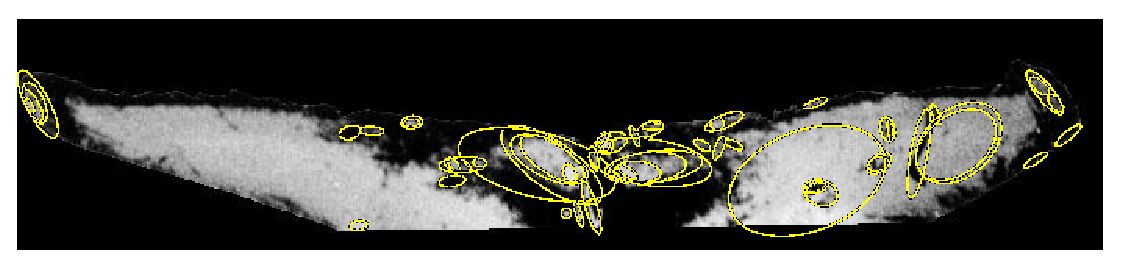
\includegraphics[width=4.0cm]{./Figs/mserTailA}}
\end{minipage}
\begin{minipage}[b]{0.48\linewidth}
  \centering
  \centerline{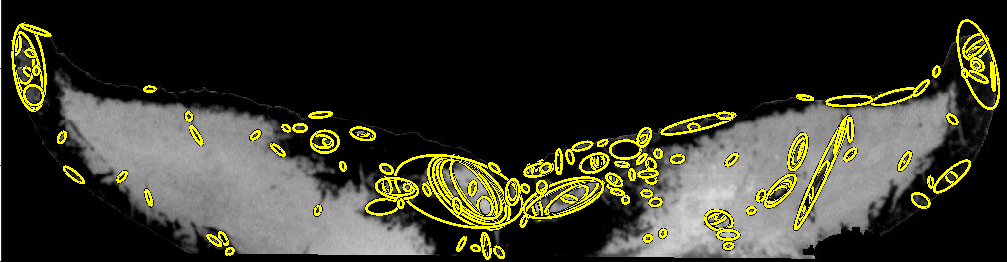
\includegraphics[width=4.0cm]{./Figs/mserTailB}}
\end{minipage}
\begin{minipage}[b]{.48\linewidth}
  \centering
  \centerline{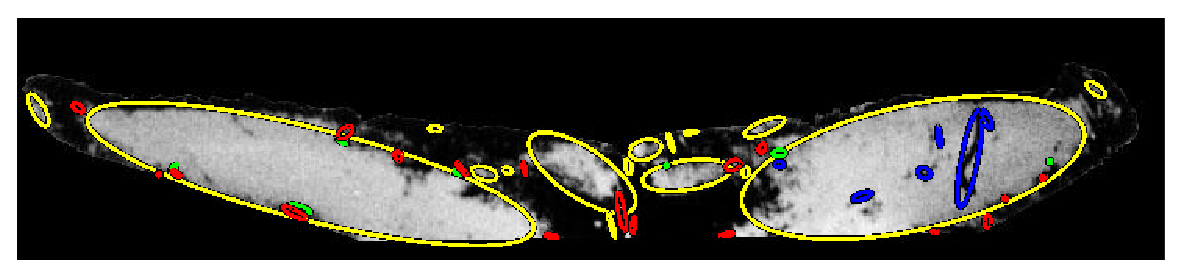
\includegraphics[width=4.0cm]{./Figs/dmsrTailA}}
\end{minipage}
\begin{minipage}[b]{0.48\linewidth}
  \centering
  \centerline{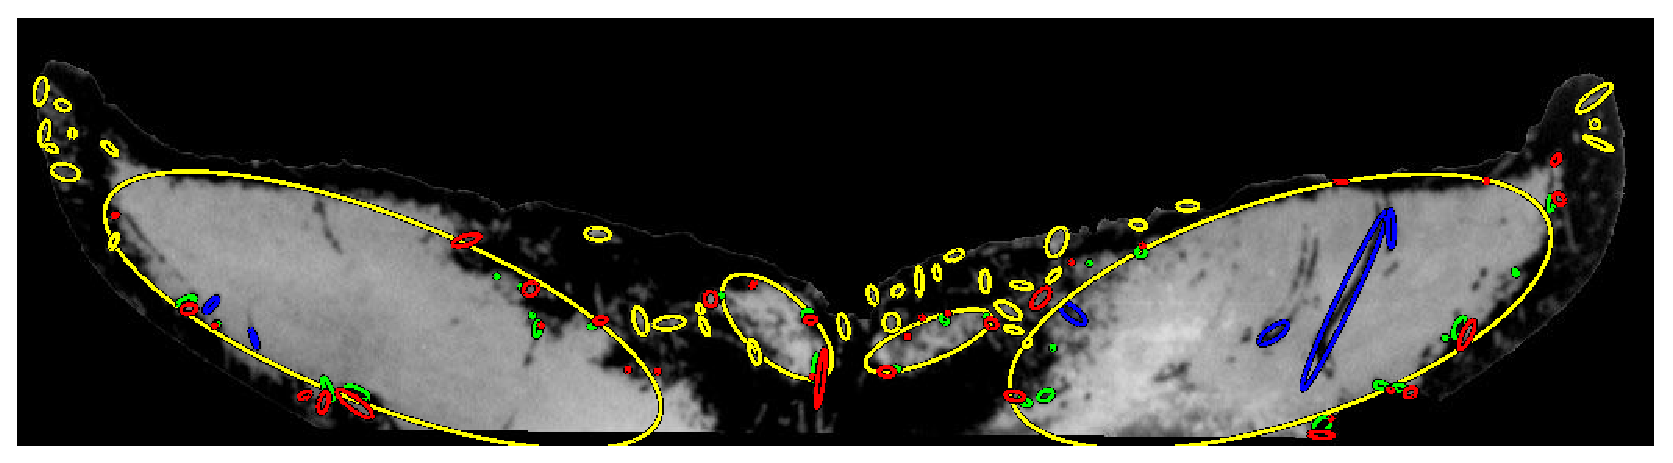
\includegraphics[width=4.0cm]{./Figs/dmsrTailB}}
\end{minipage}
 \vspace{-0.2cm}
\caption{Region detectors on two images of the tail of the same humpback whale. 
First row: MSER, second row: DMSRA.}
\label{fig:tails}
 %\vspace{-0.2cm}
\end{figure}

%----------------------------------------------------------------
\begin{figure}[htb]

\begin{minipage}[b]{.24\linewidth}
  \centering
  \centerline{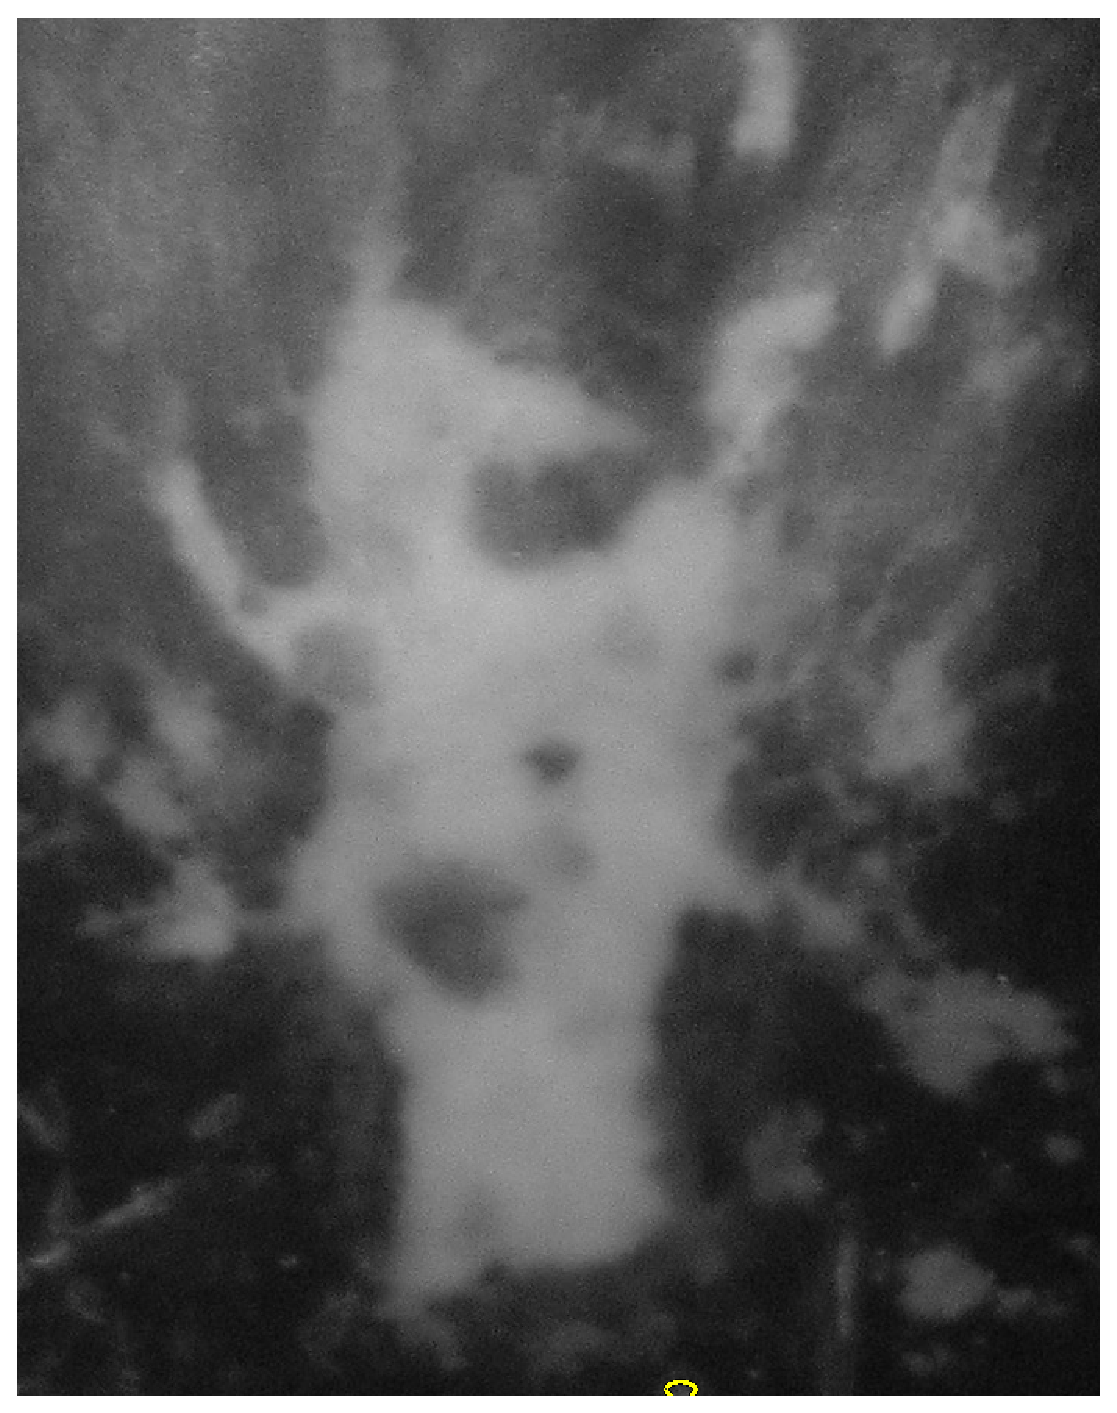
\includegraphics[height=2.0cm]{./Figs/mserLeatherbackA}}
   \centerline{(a)}\medskip
\end{minipage}
\hfill
\begin{minipage}[b]{0.24\linewidth}
  \centering
  \centerline{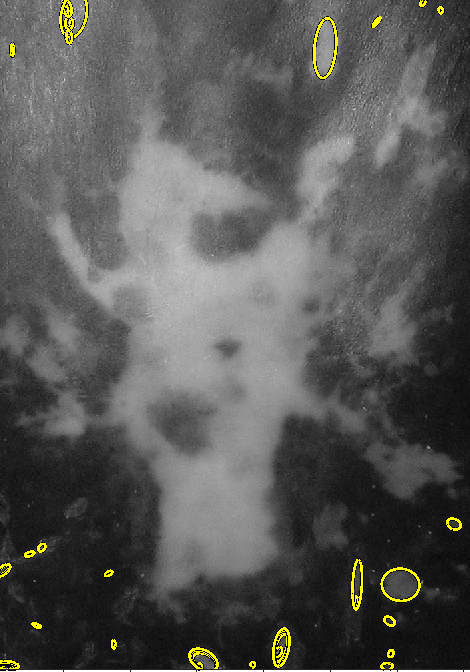
\includegraphics[height=2.2cm]{./Figs/mserLeatherbackB}}
\centerline{(b)}\medskip
\end{minipage}
\hfill
\begin{minipage}[b]{.24\linewidth}
  \centering
  \centerline{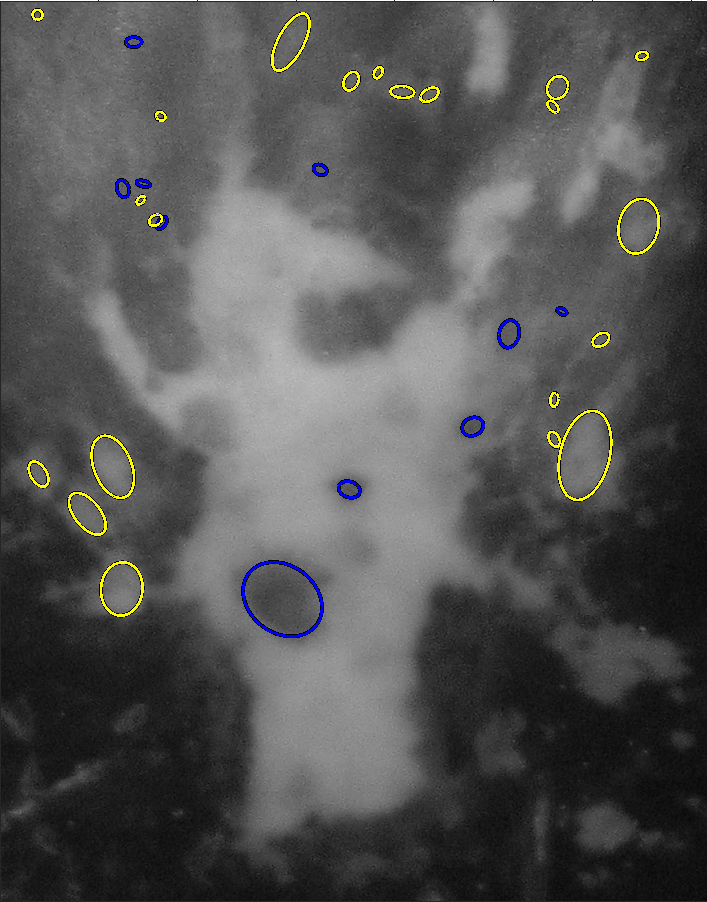
\includegraphics[height=2.0cm]{./Figs/dmsrLeatherbackA}}
\centerline{(c)}\medskip
\end{minipage}
\hfill
\begin{minipage}[b]{0.24\linewidth}
  \centering
  \centerline{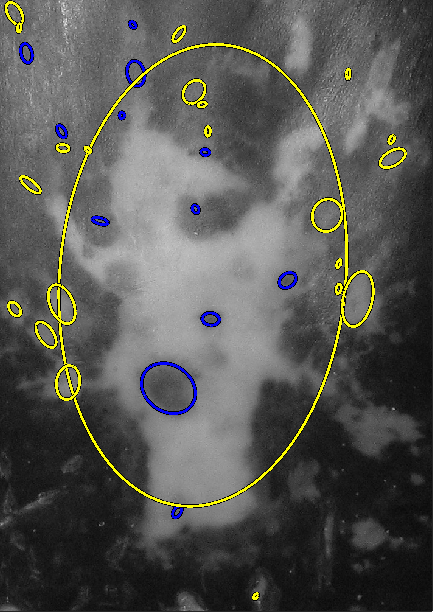
\includegraphics[height=2.2cm]{./Figs/dmsrLeatherbackB}}
 \centerline{(d)}\medskip
\end{minipage}
 \vspace{-0.4cm} 
\caption{Region detectors on two images of the pineal spot of the same leatherback turtle.
(a),(b): MSER, (c),(d): DMSR. }
\label{fig:turtle}
 \vspace{-0.2cm}
\end{figure}

A decade ago, a performance evaluation paper by the Visual Geometry Group in Oxford, compared the existing region detectors, \cite{Mikolajczyk:2005}. 
A clear conclusion of the comparison was that the {\em  Maximally Stable Extremal Regions (MSER)} is the best performing detector for {\em structured} scenes, \cite{Matas2002BMVC}. The MSER has become the de-facto standard in the field, for example as part of the MATLAB Computer Vision Systems Toolbox. Despite its success, the detector has several drawbacks: sensitivity to blur; produces many nested regions; the number of image regions is often large and the performance degrades with the resolution increase, \cite{CorRos2013}. Analysis in the geometric scale-space showed that the formulation of the stability rule makes MSER chose regular shapes, \cite{Kimmel11}.

Many researchers have proposed improvements to MSER without a drastic increase of performance. An MSER color extension, {\em Maximally Stable Color Region} outperforms an  MSER per color channel combination and a color blob detector, \cite{Forssen07}. 
Improving the MSER region distinctiveness by morphological dilation on the detected Canny edges is proposed in \cite{Wang14}. The improved detector shows better performance than MSER for bag of words classification, but the evaluation of repeatability is not reported. 
The MSER has been extended to {\em Maximally Stable Volumes} for successful segmentation of 3D medical images and paper fiber networks, \cite{DonoserB06}.

%----------------------------------------------------------------------
\begin{figure}[htb]

\begin{minipage}[b]{.48\linewidth}
  \centering
  \centerline{
\includegraphics[width=4.0cm]{./Figs/binary_marks}}

\end{minipage}
%\hfill
\begin{minipage}[b]{0.48\linewidth}
  \centering
  \centerline{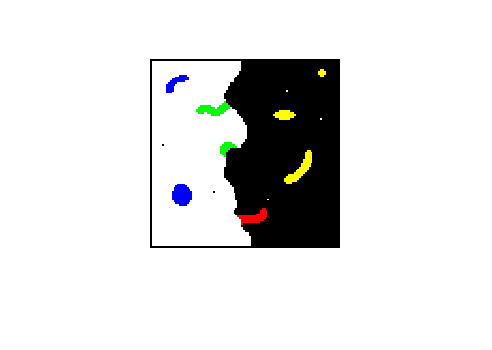
\includegraphics[width=4.0cm]{./Figs/binary_marks_clean_color_coded}}

\end{minipage}
\vspace{-0.4cm}
\caption{Binary salient regions detection.
Color coding: holes-blue, islands- yellow,
indentations - green, protrusions- red. }
\label{fig:binary_sal}
\end{figure}
\vspace*{-0.1cm}
%----------------------------------------------------------------------


Although crucial for the development of detectors, there is a shortage of evaluation benchmarks, especially for independent of the image content analysis. The standard {\em Oxford dataset} is very small: $48$ low resolution images ($6$ test sequences) with known pair homographies and evaluation protocol, \cite{Mikolajczyk:2005}.  The {\em Freiburg dataset} contains $416$ higher resolution images, generated by transforming $16$ base images in order to de-tangle transformations from content, \cite{FischerDB14}.  
The {\em TNT dataset} contains versions of viewpoint sequences with increasing resolution from $1.5$ MB to $8$ MB, and highly accurate homographies. It is suitable for evaluating robustness to resolution rather than transformations \cite{CorRos2013}. 

This paper contributes to solving the identified problems. A new regions detector, the {\em Data-driven Morphology Salient Regions (DMRS)} is proposed and available open source, \cite{Rang:software}. It is related to the {\em Morphology-based Stable Salient Regions (MSSR)} detector we have developed in the context of humpback whale identification, \cite{RangMSSR06, RangHumpb06}. DMRS  includes a robust to lighting and blur binarization, leading to much smaller and more stable number of regions. It has comparable or higher (lighting, blur and increased resolution) repeatability to MSER while detecting non-redundant perceptually salient regions, see Fig.\ref{fig:tails}. Figure \ref{fig:turtle} illustrates that MSER does not find useful regions on the leatherback images, unlike the DMSR. A new dataset, OxFrei', combining the natural homographies of the Oxford and the higher resolution images of the Freiburg datasets, is introduced, \cite{Rang:dataset}.

\section{Data-driven Morphology Salient Regions Detection}
\label{sec:DMSR}

The MSER and MSSR decompose a gray-scale image into binary cross-sections and evaluate the stability of the CCs or accumulate saliency masks, respectively. DMSR starts with a data-driven binarization, producing single binary image transforming the problem into binary saliency.

%----------------------------------------------------------------------
\begin{table}[hbt]
\begin{minipage}[b]{0.98\linewidth}\begin{tabular}{|l l|}
\hline

{\bf ISS} & A CC $S^i_{fb} = \{\p \in \mcD, \forall \p=f,$\\&$\forall \q \in \partial S^i_{fb}, \q=b, \q \notin \partial \B $ \},\\
$2$ types & $S^i_{10}$ (islands), $S^i_{01}$  (holes); $\S^i = S_{01}^i \cup S_{10}^i$\\
{\bf BSS} &  $S_{fb}^b: \{\p \in S_{fb}^b \subset{\cal B}^f, \forall \p = f,$\\&$ \q \in \partial S_{fb}^b \subset {\partial \cal B}^f,\forall \q = b \}$, \\
& $|\partial {\cal B}^f| - |\partial ({\cal B}^f \backslash S_{fb}^b)| < 2 \pi r$\\
$2$ types & $S^b_{10}$ (protr.), $S^b_{01}$ (indent.); $\S^b = S_{01}^b \cup S_{10}^b$\\
{\bf Regions} &  $\S = \S^i$ (DMSR), $\S = \S^i \cup \S^b$ (DMSRA)  \\

\hline
\end{tabular}
\caption{Binary saliency definitions used in Section \ref{ssec:binary}.}\label{table:binary_sal}
\end{minipage}
\vspace*{-0.1cm}
\end{table}


\subsection{Binary Salient Regions Detection}
\label{ssec:binary}
The claim is that the perceptual saliency in a binary image of a structured scene 
 $\B: \mcD \subset \mathcal{Z}^2 \rightarrow \{0,1\}$ (1-white, 0-black)
is only due to the spatial layout of the image regions. 
There are  $4$ possible types of salient regions. The $2$ types of {\em inner salient structures (ISS)} are {\em holes} - set of connected black pixels entirely surrounded by white pixels and the inverted {\em islands}- set of connected white pixels surrounded by black ones. A significant connected component (CC) ${\cal B}^1$ is defined as a CC with area proportional to the image area by $\Lambda$. The radius of the morphological structuring element is $r$ and  the area opening parameter for  noise filtering is $\lambda$. The $2$ {\em boundary salient structures (BSS)} are the {\em protrusions}- set of white pixels on the border of a significant CC, which if pinched off from the CC, will increase its boundary with no more than $2\pi r$ and the inverted {\em indentations}. 


The types are also valid for the MSSR detector. The regions are obtained from $\B$ by morphological operations: hole filling, top hat and area opening, for details see \cite{RangMSSR06, RangHumpb06}. The ISS are similar to the definition of the MSER+ and MSER- regions, \cite{Matas2002BMVC}. In this paper, detectors using only ISS (e.g. directly comparable to MSER) are denoted by DMSR/MSSR, while DMSRA/MSSRA are detectors using all region types. These definitions are summarized in Table \ref{table:binary_sal} and the exact shape regions on a synthetic $100 \times 100$ binary image with parameters $\Lambda=100$, $r=5$ and $\lambda = 10$  are shown on Fig.\ref{fig:binary_sal}.

\subsection{Data-driven binarization}
\label{ssec:binarize}
Any gray-scale image  $\I: \mcD \subset \mathcal{Z}^2 \rightarrow \mcT $ ($\mcT = \{0,1, ..., t_{max}\}$, $t_{max} = 2^n-1$ is the maximum
gray value encoded by $n$ bits; usually $n=8$, $t_{max} = 256$) can be decomposed into cross-sections at
every possible level $t$:  $\I = \sum_{t \in \mcT}CS_t(\I)$, 
($CS_0(\I) = \I$). Obtaining a cross-section at level $t$ is equivalent to thresholding the image at threshold $t$ (setting all pixels with values below $t$ to $0$ and the ones above- to $1$), $CS_t(\I)$ is a binary image. 
Three groups of CC are defined: $\mcA_t$- {\em all} CC in $CS_t(\I)$, $\mcL_t$- the {\em large} CC in $CS_t(\I)$ and 
$\mcV_t$- the {\em very large} CC in $CS_t(\I)$.  The size of each CC is categorized using $\Lambda_{\mcL}$ and $\Lambda_{\mcV}$ fraction of the image area $A_{\I}$. Lets denote the normalized number of elements in a set by $\Vert \cdot \Vert = |\cdot| / \max_{t \in \mcT}|\cdot|$
Finding the optimal threshold $t_{opt}$ is then defined as
%\begin{equation*}
$t_{opt} = \argmax_{t \in \mcT}( w^{\mcA} \Vert \mcA_t \Vert + w^{\mcL} \Vert \mcL_t \Vert + w^{\mcV} \Vert \mcV_t \Vert )$,
%\end{equation*}
where $w^{\cdot}$ are the weights per set of CCs.  

The standard Otsu thresholding does not provide criterion for selecting a single stable $CS$, while choosing the threshold $t_{opt}$ ensures stable number of regions across transformations, see figs. \ref{fig:binary_hist} and \ref{fig:leuven_bin} for lighting.
%------------------------------------------------------------------------
%\vspace{-0.5cm}
\begin{figure}[htb]

\begin{minipage}[b]{0.49\linewidth}
  \centering
  \centerline{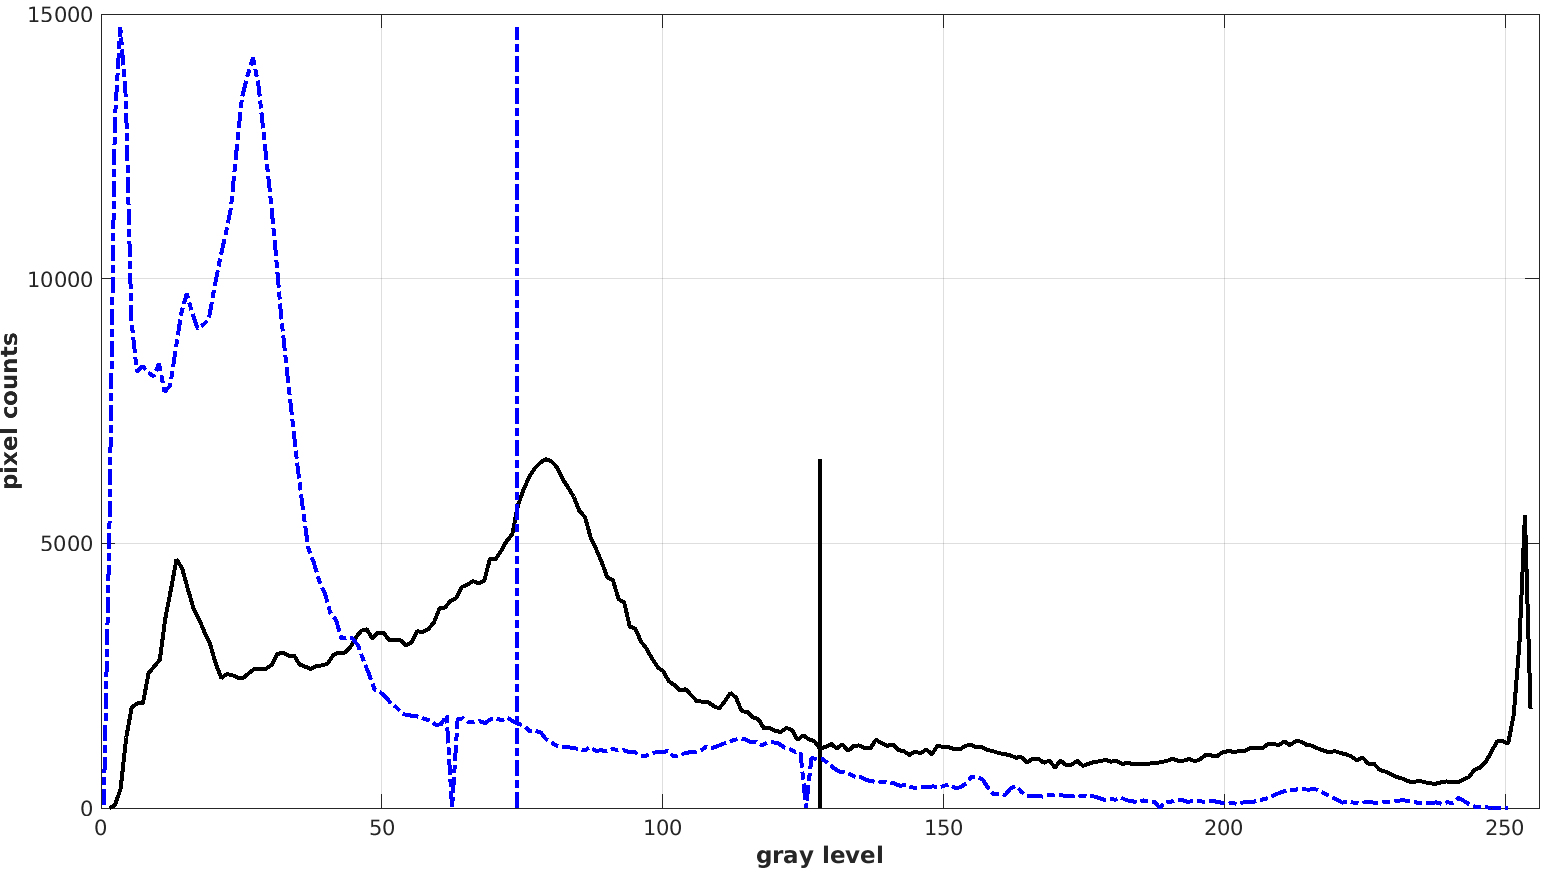
\includegraphics[width=4.3cm]{./Figs/hist_otsu_leuven_1_4}}
  \centerline{(a) Otsu}\medskip
\end{minipage}
\hfill
%\vspace{-0.5cm}
\begin{minipage}[b]{0.49\linewidth}
  \centering
  \centerline{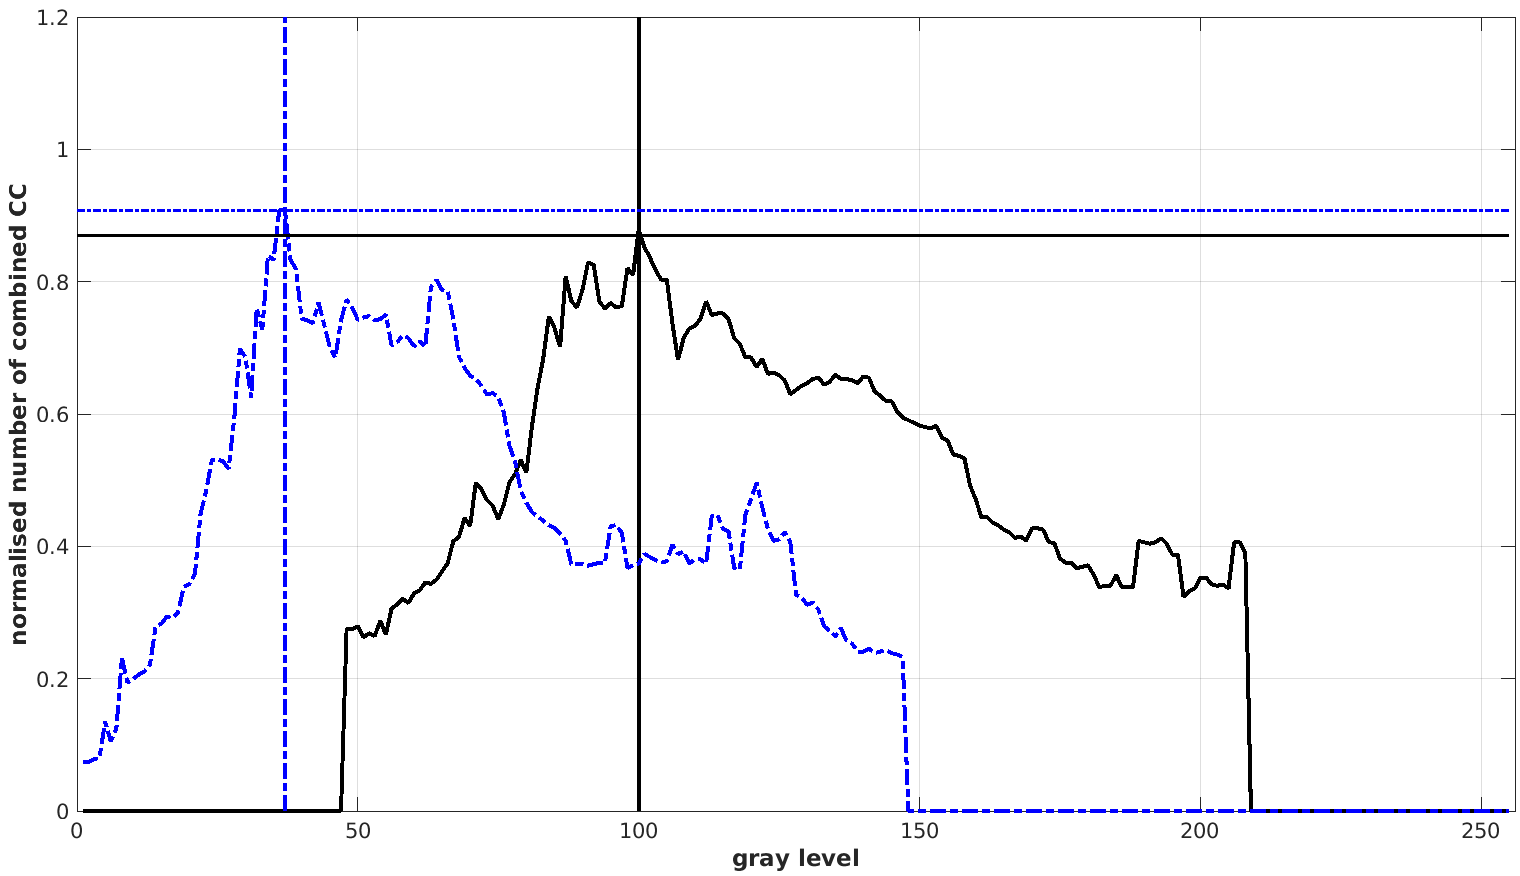
\includegraphics[width=4.3cm]{./Figs/hist_numcc_leuven_1_4}}
\centerline{(b) Max number CC}\medskip
\end{minipage}
\hfill
\vspace{-0.5cm}
\caption{Finding the optimal threshold for $2$ images from the 'Leuven' sequence 
(Oxford dataset, lighting): the base image - solid black line, the 4th image - dotted blue line.}
\label{fig:binary_hist}
%
\end{figure}
%------------------------------------------------------------------------
%\vspace{-0.5cm}

\begin{figure}[htb]

\begin{minipage}[b]{.3\linewidth}
  \centering
  \centerline{\includegraphics[width=2.8cm]{./Figs/leuven1}}
%  \vspace{1.5cm}
%   \centerline{(a)}\medskip
\end{minipage}
\hfill
\begin{minipage}[b]{0.3\linewidth}
  \centering
  \centerline{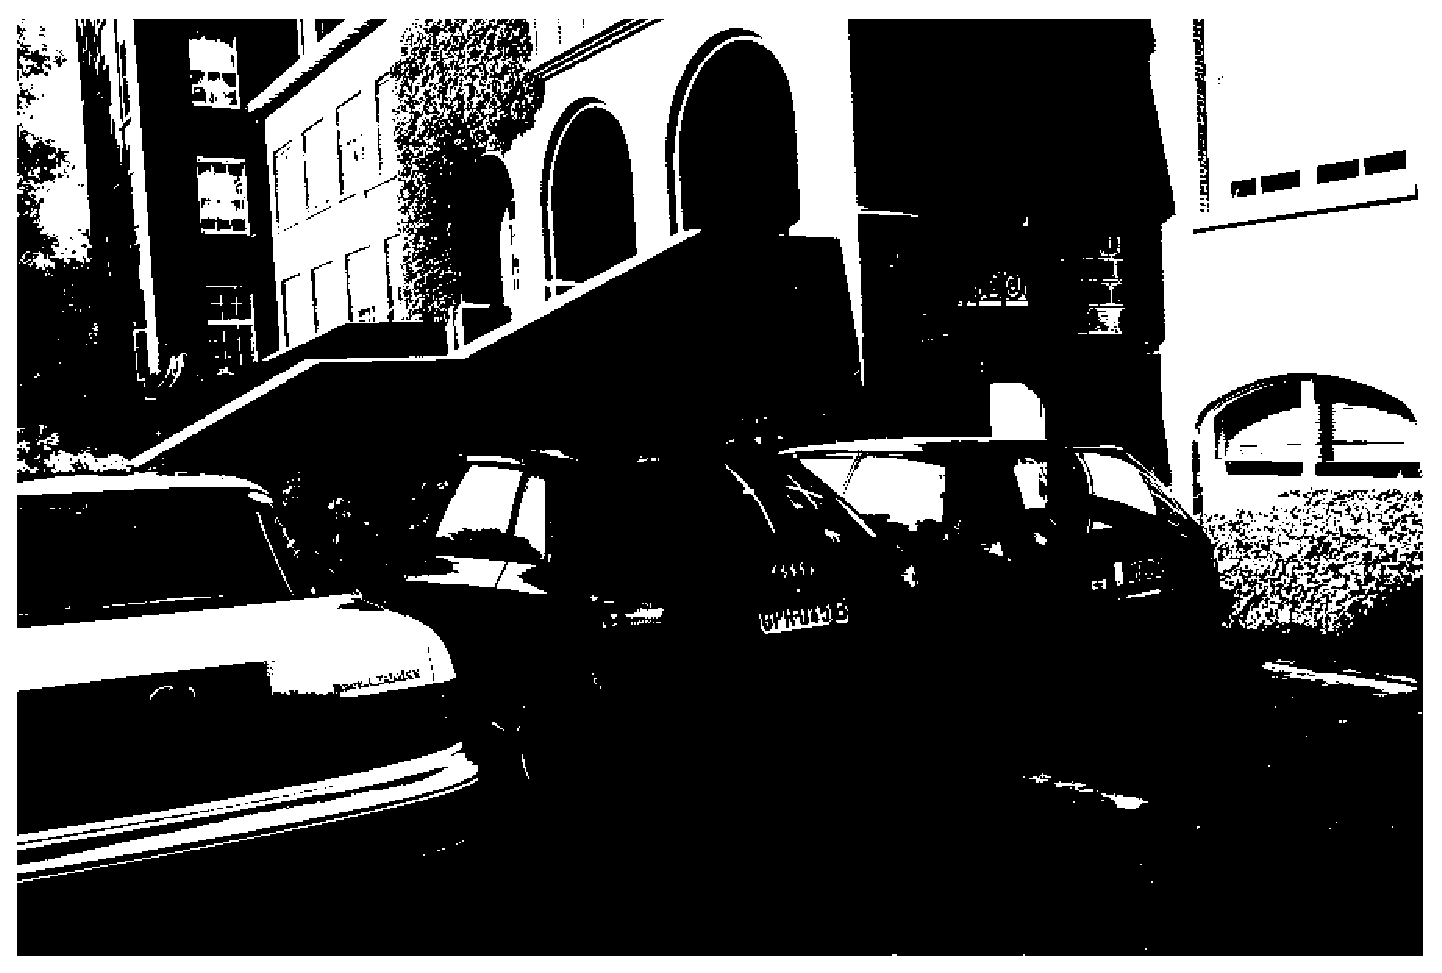
\includegraphics[width=2.7cm]{./Figs/leuven1_otsu}}
%  \vspace{1.5cm}
  % \centerline{(b)}\medskip
\end{minipage}
\hfill
\begin{minipage}[b]{0.3\linewidth}
  \centering
  \centerline{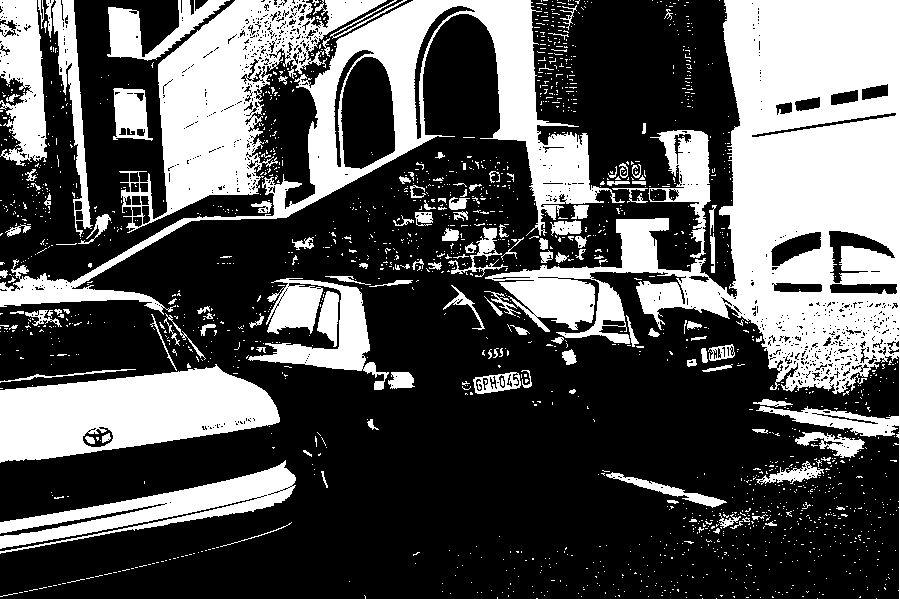
\includegraphics[width=2.7cm]{./Figs/leuven1_numcc}}
%  \vspace{1.5cm}
  % \centerline{(c)}\medskip
\end{minipage}

\begin{minipage}[b]{.3\linewidth}
  \centering
  \centerline{\includegraphics[width=2.7cm]{./Figs/leuven4}}
%  \vspace{1.5cm}
   \centerline{(a)}\medskip
\end{minipage}
\hfill
\begin{minipage}[b]{0.3\linewidth}
  \centering
  \centerline{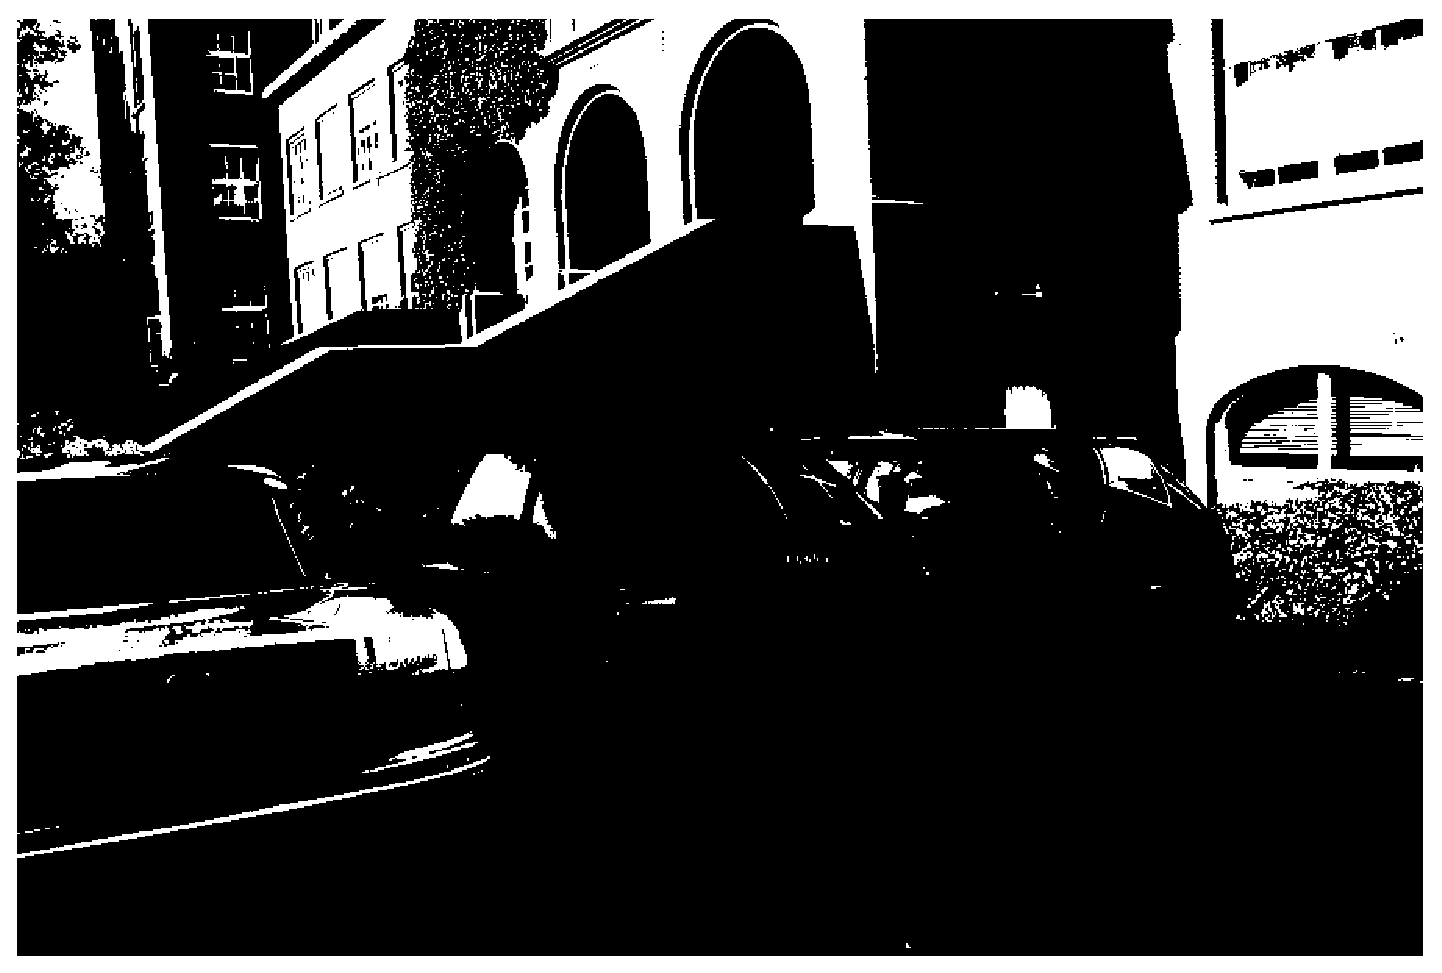
\includegraphics[width=2.7cm]{./Figs/leuven4_otsu}}
%  \vspace{1.5cm}
   \centerline{(b)}\medskip
\end{minipage}
\hfill
\begin{minipage}[b]{0.3\linewidth}
  \centering
  \centerline{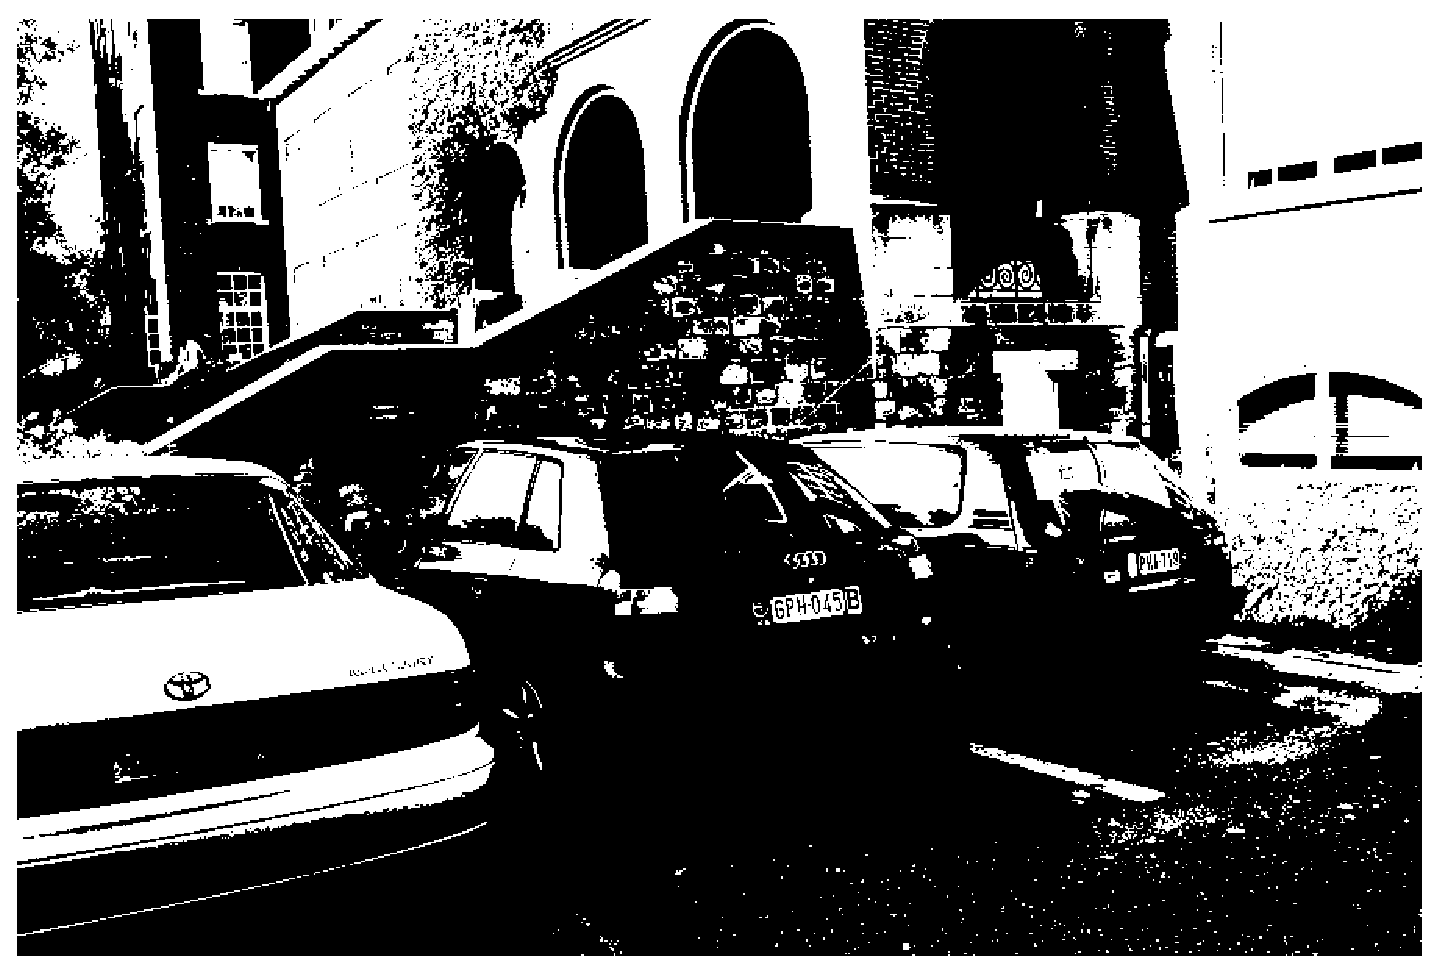
\includegraphics[width=2.7cm]{./Figs/leuven4_numcc}}
%  \vspace{1.5cm}
   \centerline{(c)}\medskip
\end{minipage}

 \vspace{-0.5cm}
\caption{Binarization of $2$ images of the 'Leuven' sequence (lighting). Top row- base image, bottom row- $4$th image; (a) gray scale; (b) Otsu binarization, (c) proposed binarization.}
\label{fig:leuven_bin}
%
\end{figure}
%------------------------------------------------------------------------

After the data-driven binarization, the DMSR detector finds the set of affine-covariant regions $\S$ from the single binary image $CS_{t_{opt}}$ as described in section \ref{ssec:binary} and \cite{RangMSSR06, RangHumpb06}. DMSR produces smaller number of non-overlapping and perceptually salient regions (visualized by their equivalent ellipses, not exact shapes) compared to MSER, Figs. \ref{fig:det_graffiti} and \ref{fig:wood}.

\section{Performance  Evaluation}
\label{sec:perf}
The {\em repeatability score} ($R$) and the {\em number of correspondences} ($N_C$) are the main performance evaluation measures, \cite{Mikolajczyk:2005}. The maximum overlap error between matching regions is $40\%$. The $R$ score between a pair of images (base, transf.) $(\I_B,\I_T)$ is the ratio between $N_C$ in the common image part and the smaller number of regions in the pair. The structured scenes from each dataset are considered and $5$ detectors are evaluated: MSER, MSSR(A) and DMSR(A). The MSER software is used with its default settings and the (D)MSSR(A) parameters are: $r = 0.02*\sqrt{A_{\I} / \pi}$, $\lambda=3r$ ,$\Lambda_{\mcL}=0.001$, $\Lambda_{\mcV}=0.01$ and  $w^{\cdot}=0.33$.  
All regions and performance plots on all data and detectors are available online, \cite{Rang:html_res}.

%------------------------------------------------------------------------
\begin{figure}[htb]

\begin{minipage}[b]{.49\linewidth}
  \centering
  \centerline{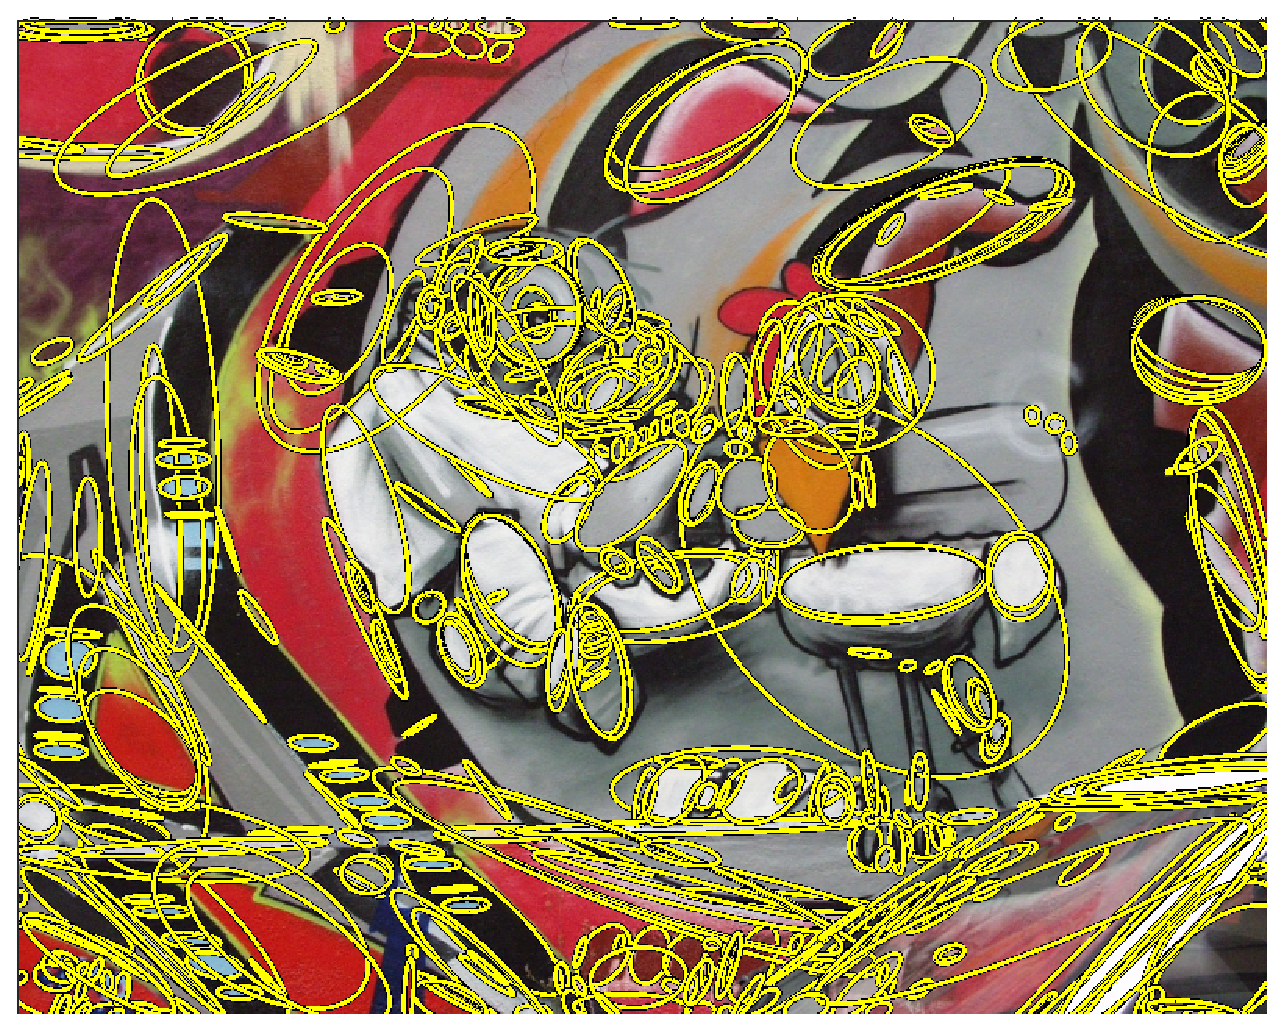
\includegraphics[width=4.0cm]{./Figs/mserGraffiti1}}
 % \vspace{0.2cm}
 % \centerline{(a) MSER}\medskip
\end{minipage}
\hfill
\begin{minipage}[b]{0.49\linewidth}
  \centering
  \centerline{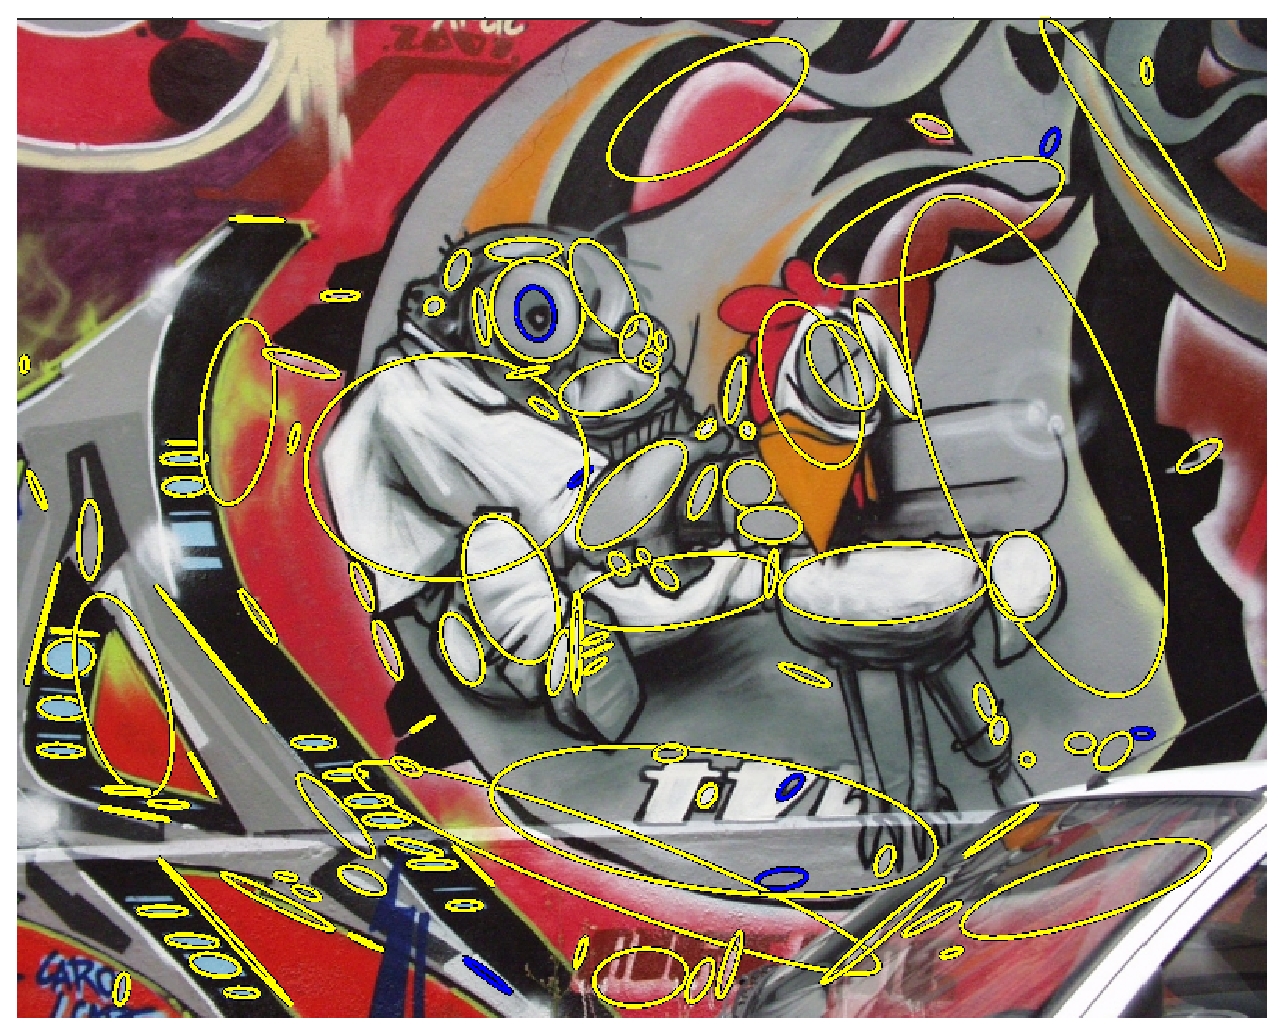
\includegraphics[width=4.0cm]{./Figs/dmsrGraffiti1}}
 % \vspace{0.2cm}
 % \centerline{(b) DMSR}\medskip
\end{minipage}
\vspace{-0.25cm}
\caption{Salient region detectors on the base image of 'Graffiti' sequence, Oxford dataset. Left: MSER, right: DMSR}
\label{fig:det_graffiti}
%
\end{figure}
%------------------------------------------------------------------------
\begin{figure}[htb]

\begin{minipage}[b]{.49\linewidth}
  \centering
  \centerline{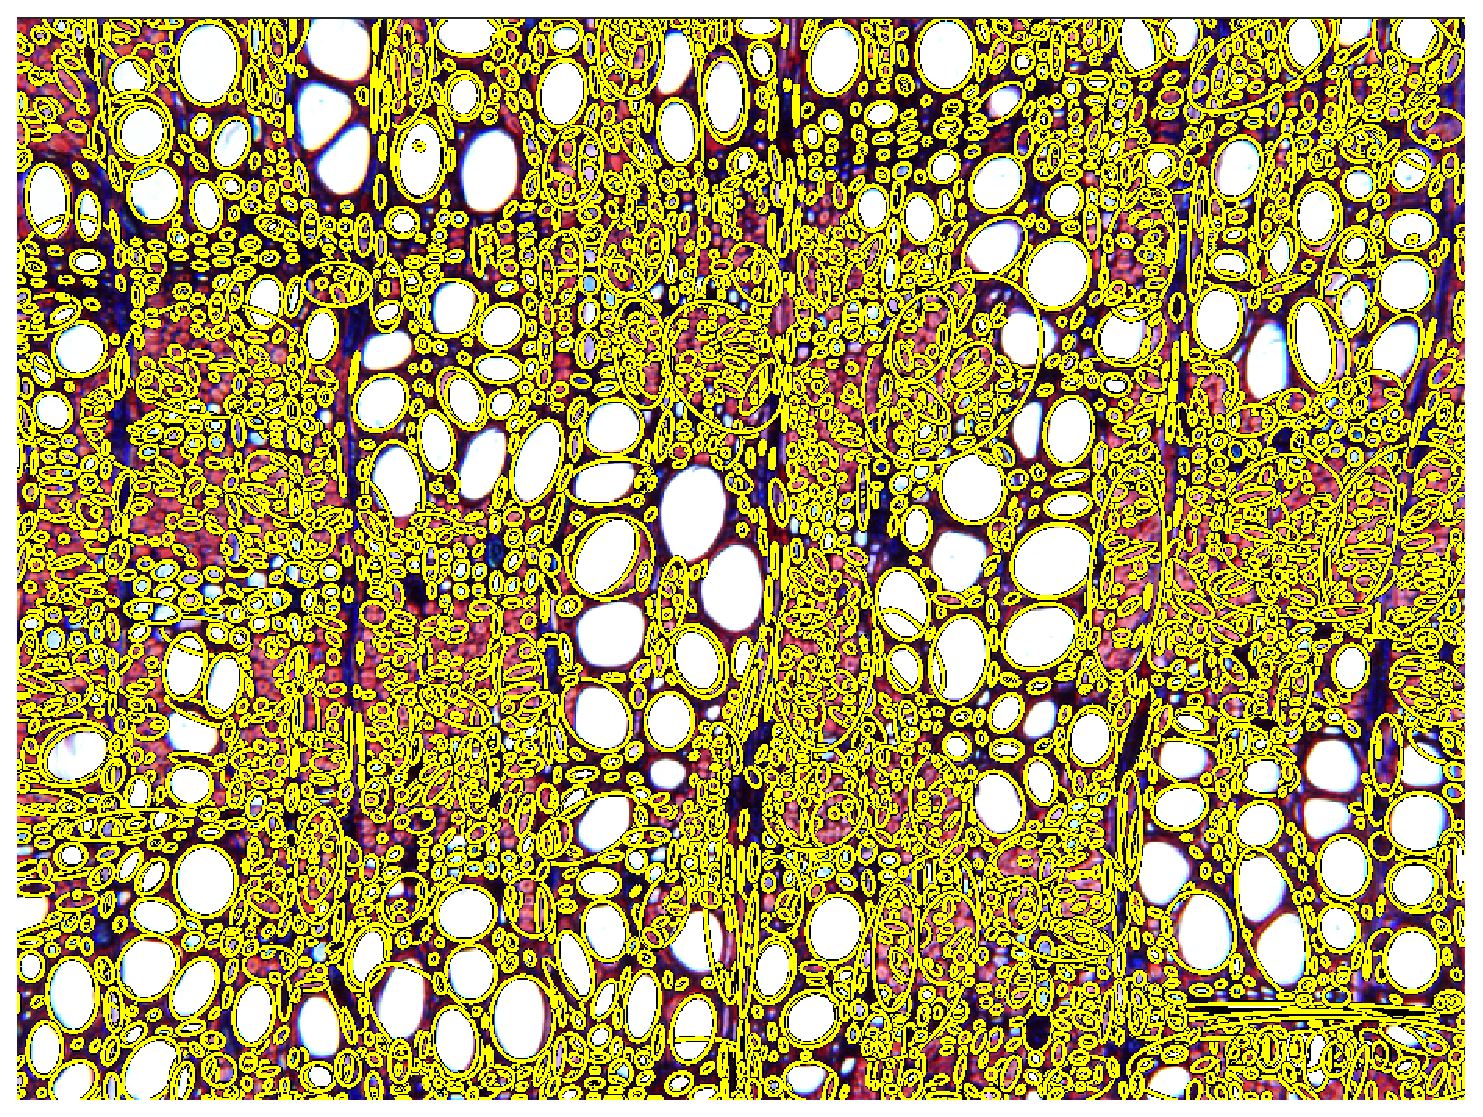
\includegraphics[width=4.0cm]{./Figs/mserWood}}
 % \vspace{0.2cm}
 % \centerline{(a) MSER}\medskip
\end{minipage}
\hfill
\begin{minipage}[b]{0.49\linewidth}
  \centering
  \centerline{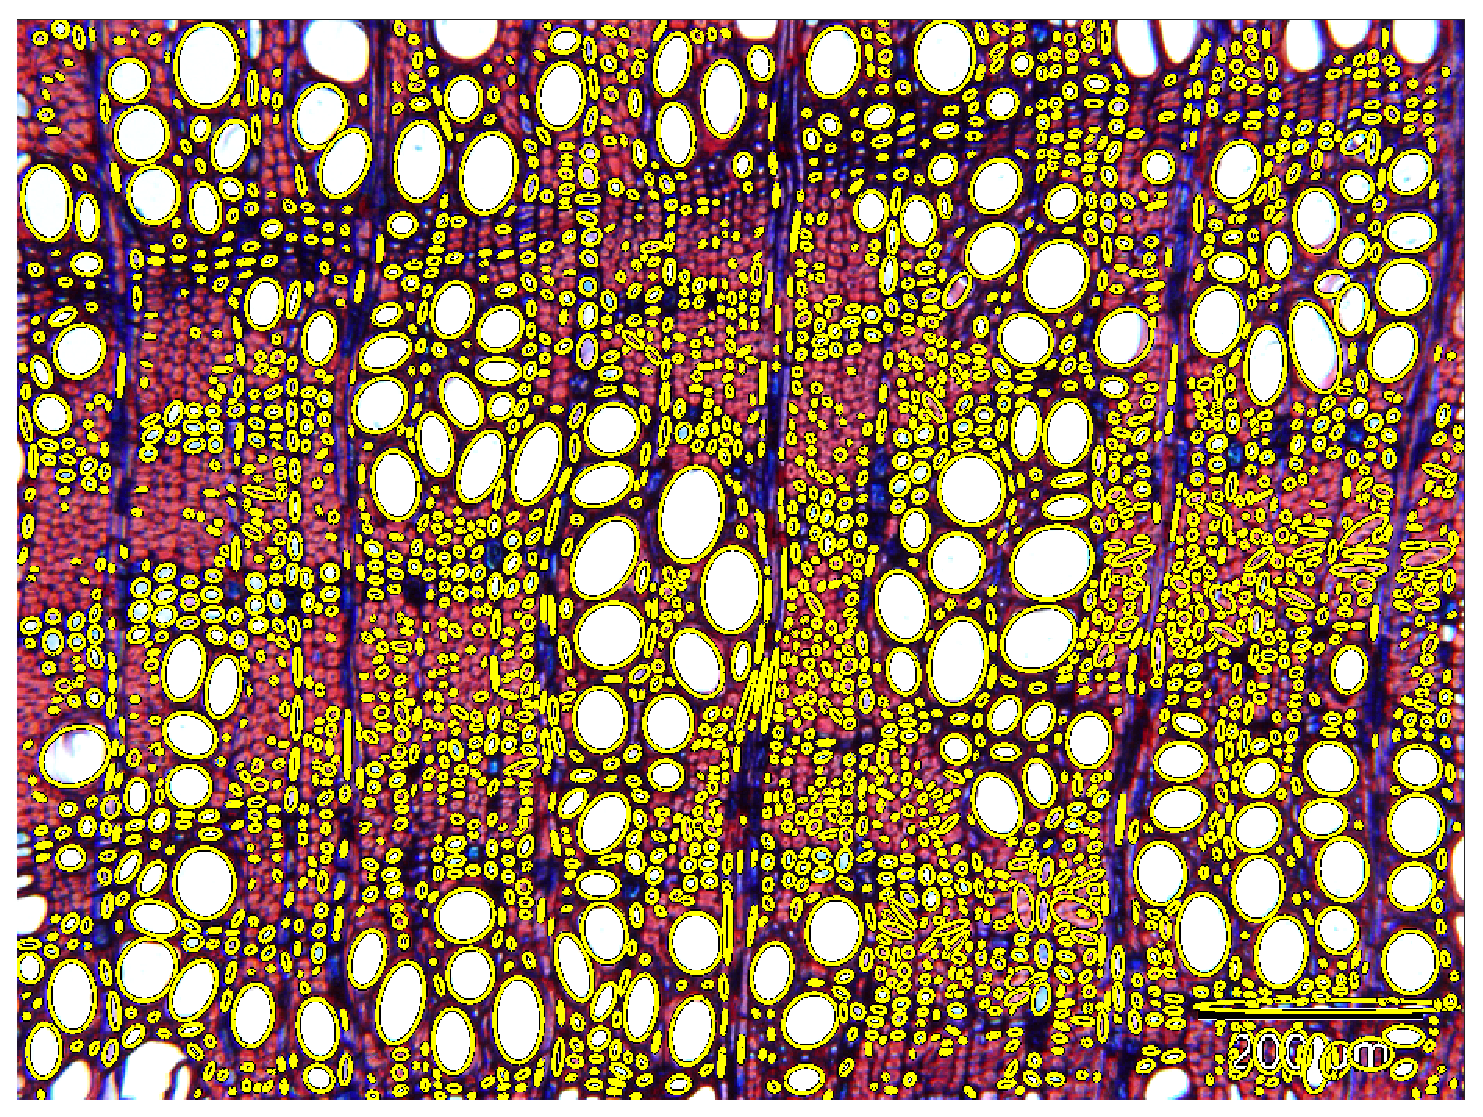
\includegraphics[width=4.0cm]{./Figs/dmsrWood}}
 % \vspace{0.2cm}
 % \centerline{(b) DMSR}\medskip
\end{minipage}
%\vspace{-0.25cm}
\caption{Salient region detectors on microscopy wood images. Left: MSER (every second region is shown), right: DMSR}
\label{fig:wood}
%
\end{figure}
%\vspace{-0.5cm}
%------------------------------------------------------------------------
\begin{figure}[htb]
\centering
\begin{minipage}[b]{.99\linewidth}
  \centering
  \centerline{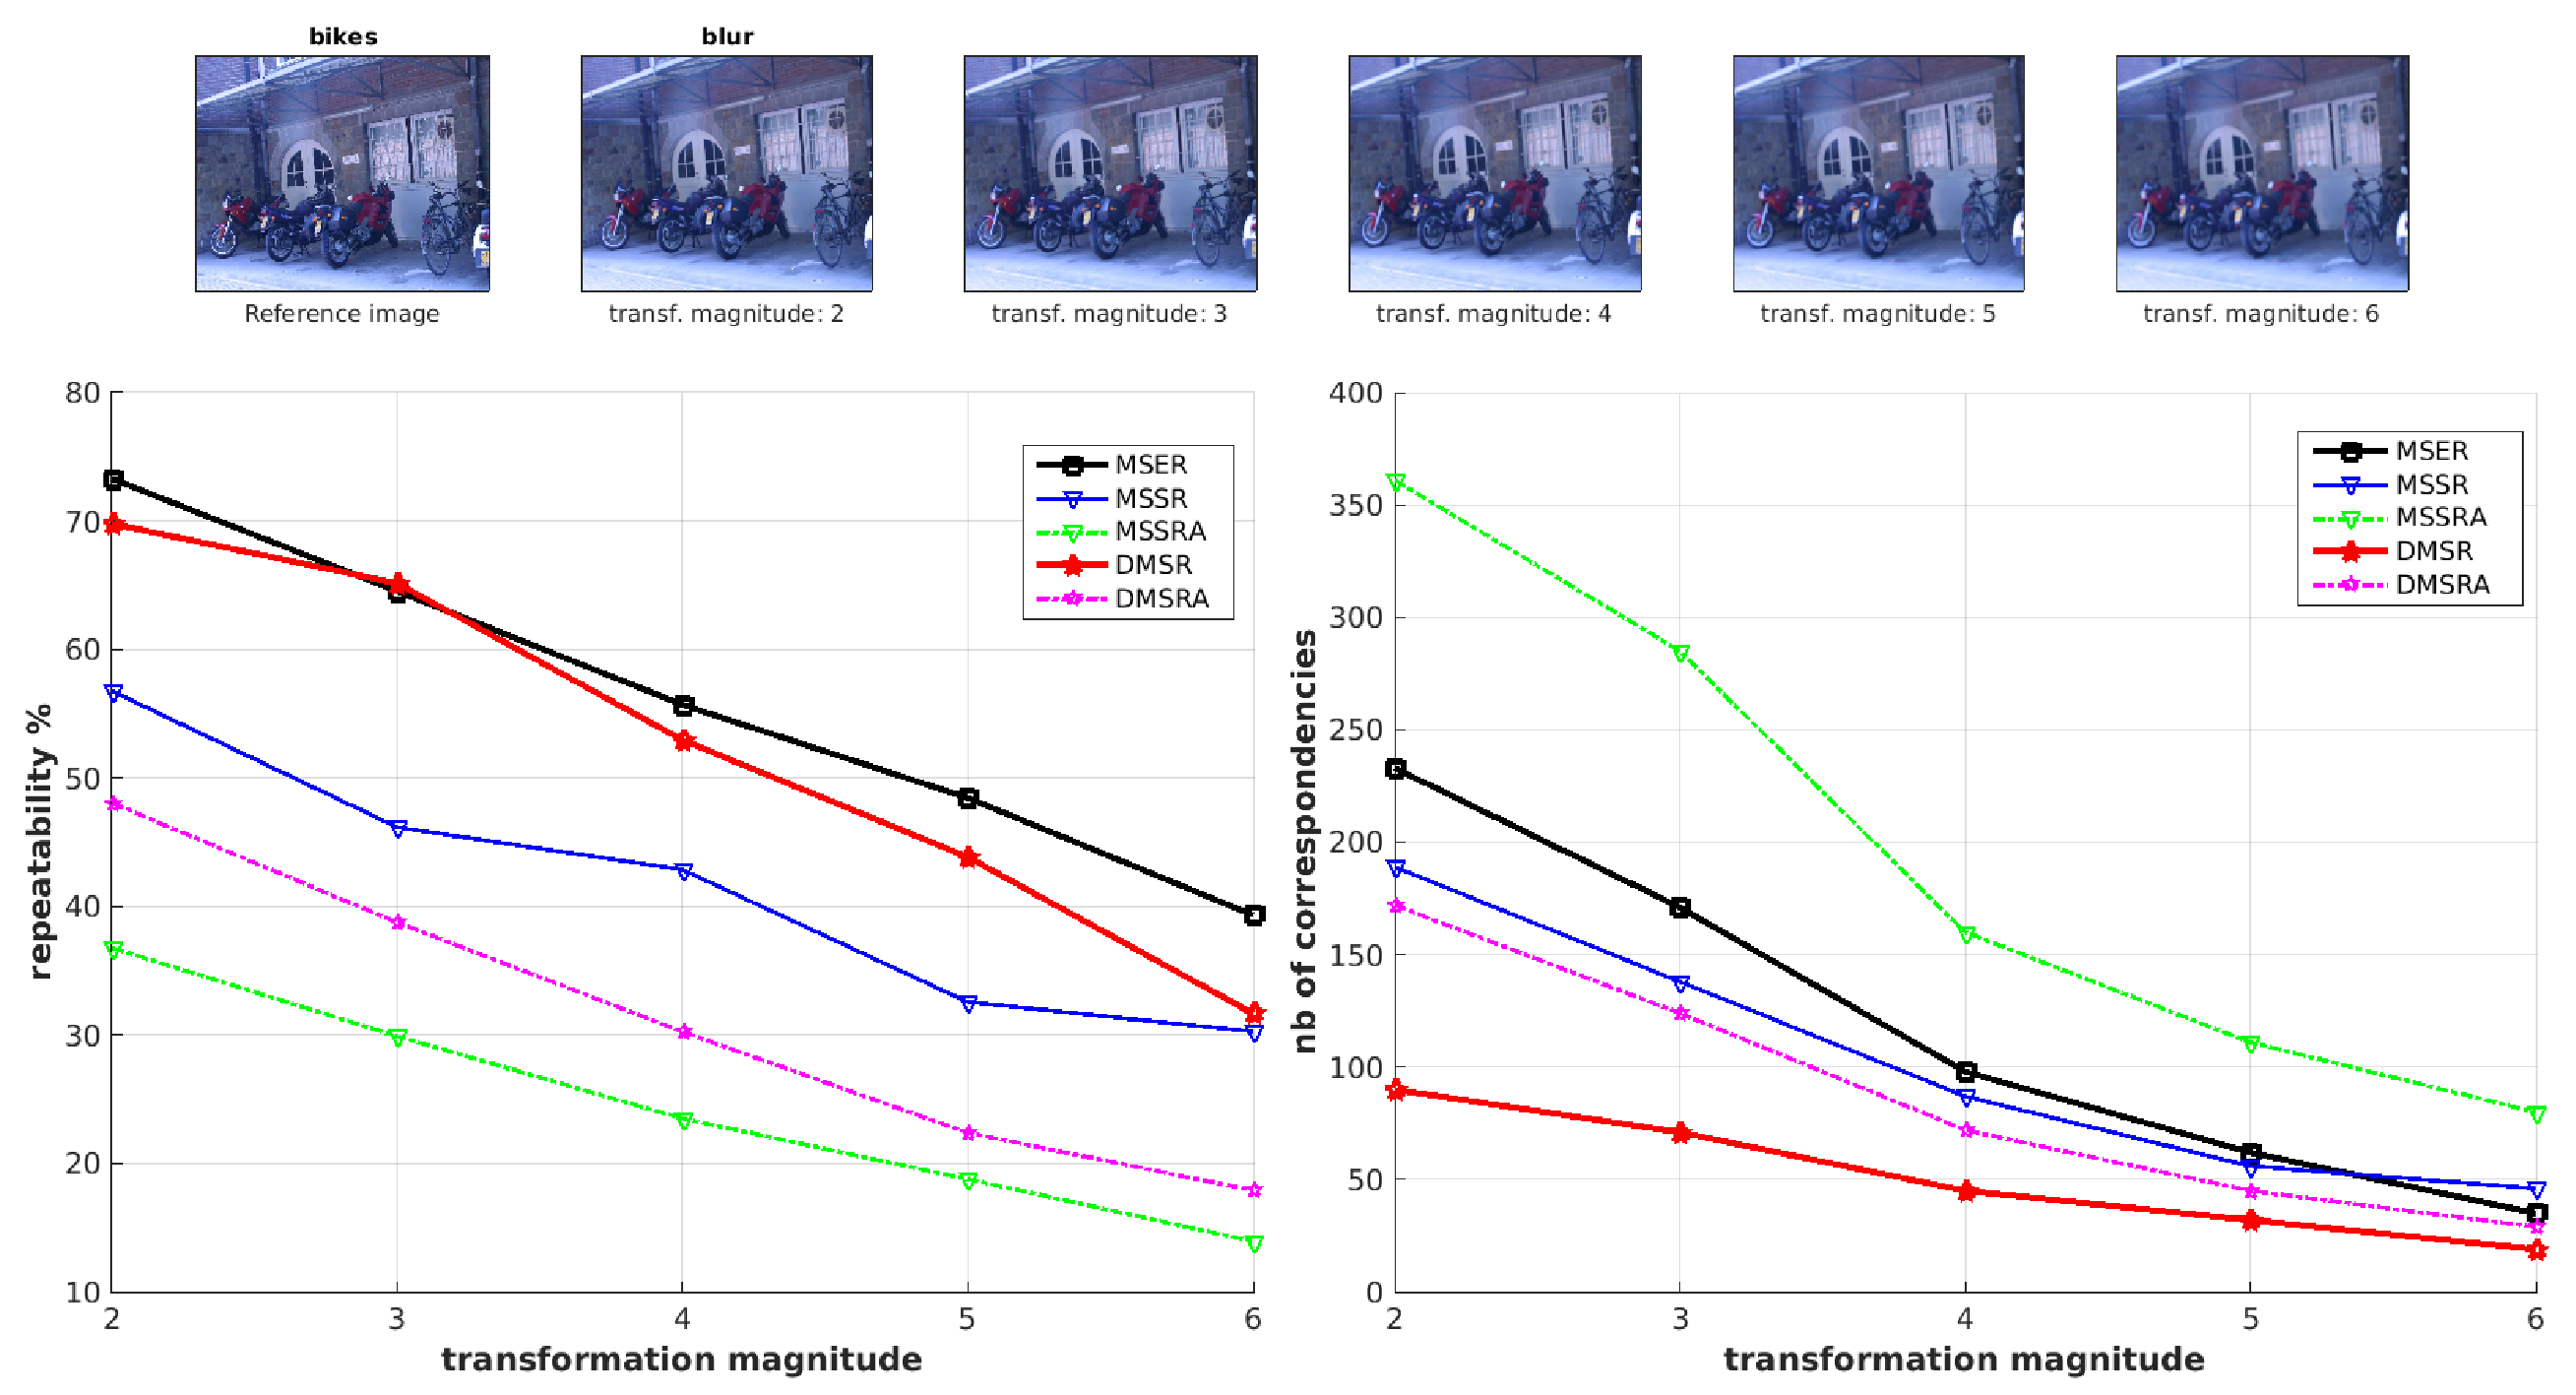
\includegraphics[width=8.4cm]{./Figs/repeatability_all_affine_bikes_blur}}
 % \vspace{0.2cm}
 % \centerline{(a) MSER}\medskip
\end{minipage}
\hfill
%\vspace{-0.25cm}
\caption{Region detectors on 'Bikes', Oxford dataset.}
\label{fig:det_bikes}
%
\end{figure}
%------------------------------------------------------------------------
%\vspace{-0.5cm}
\begin{figure}[htb]
\centering
\begin{minipage}[b]{.99\linewidth}
  \centering
 \centerline{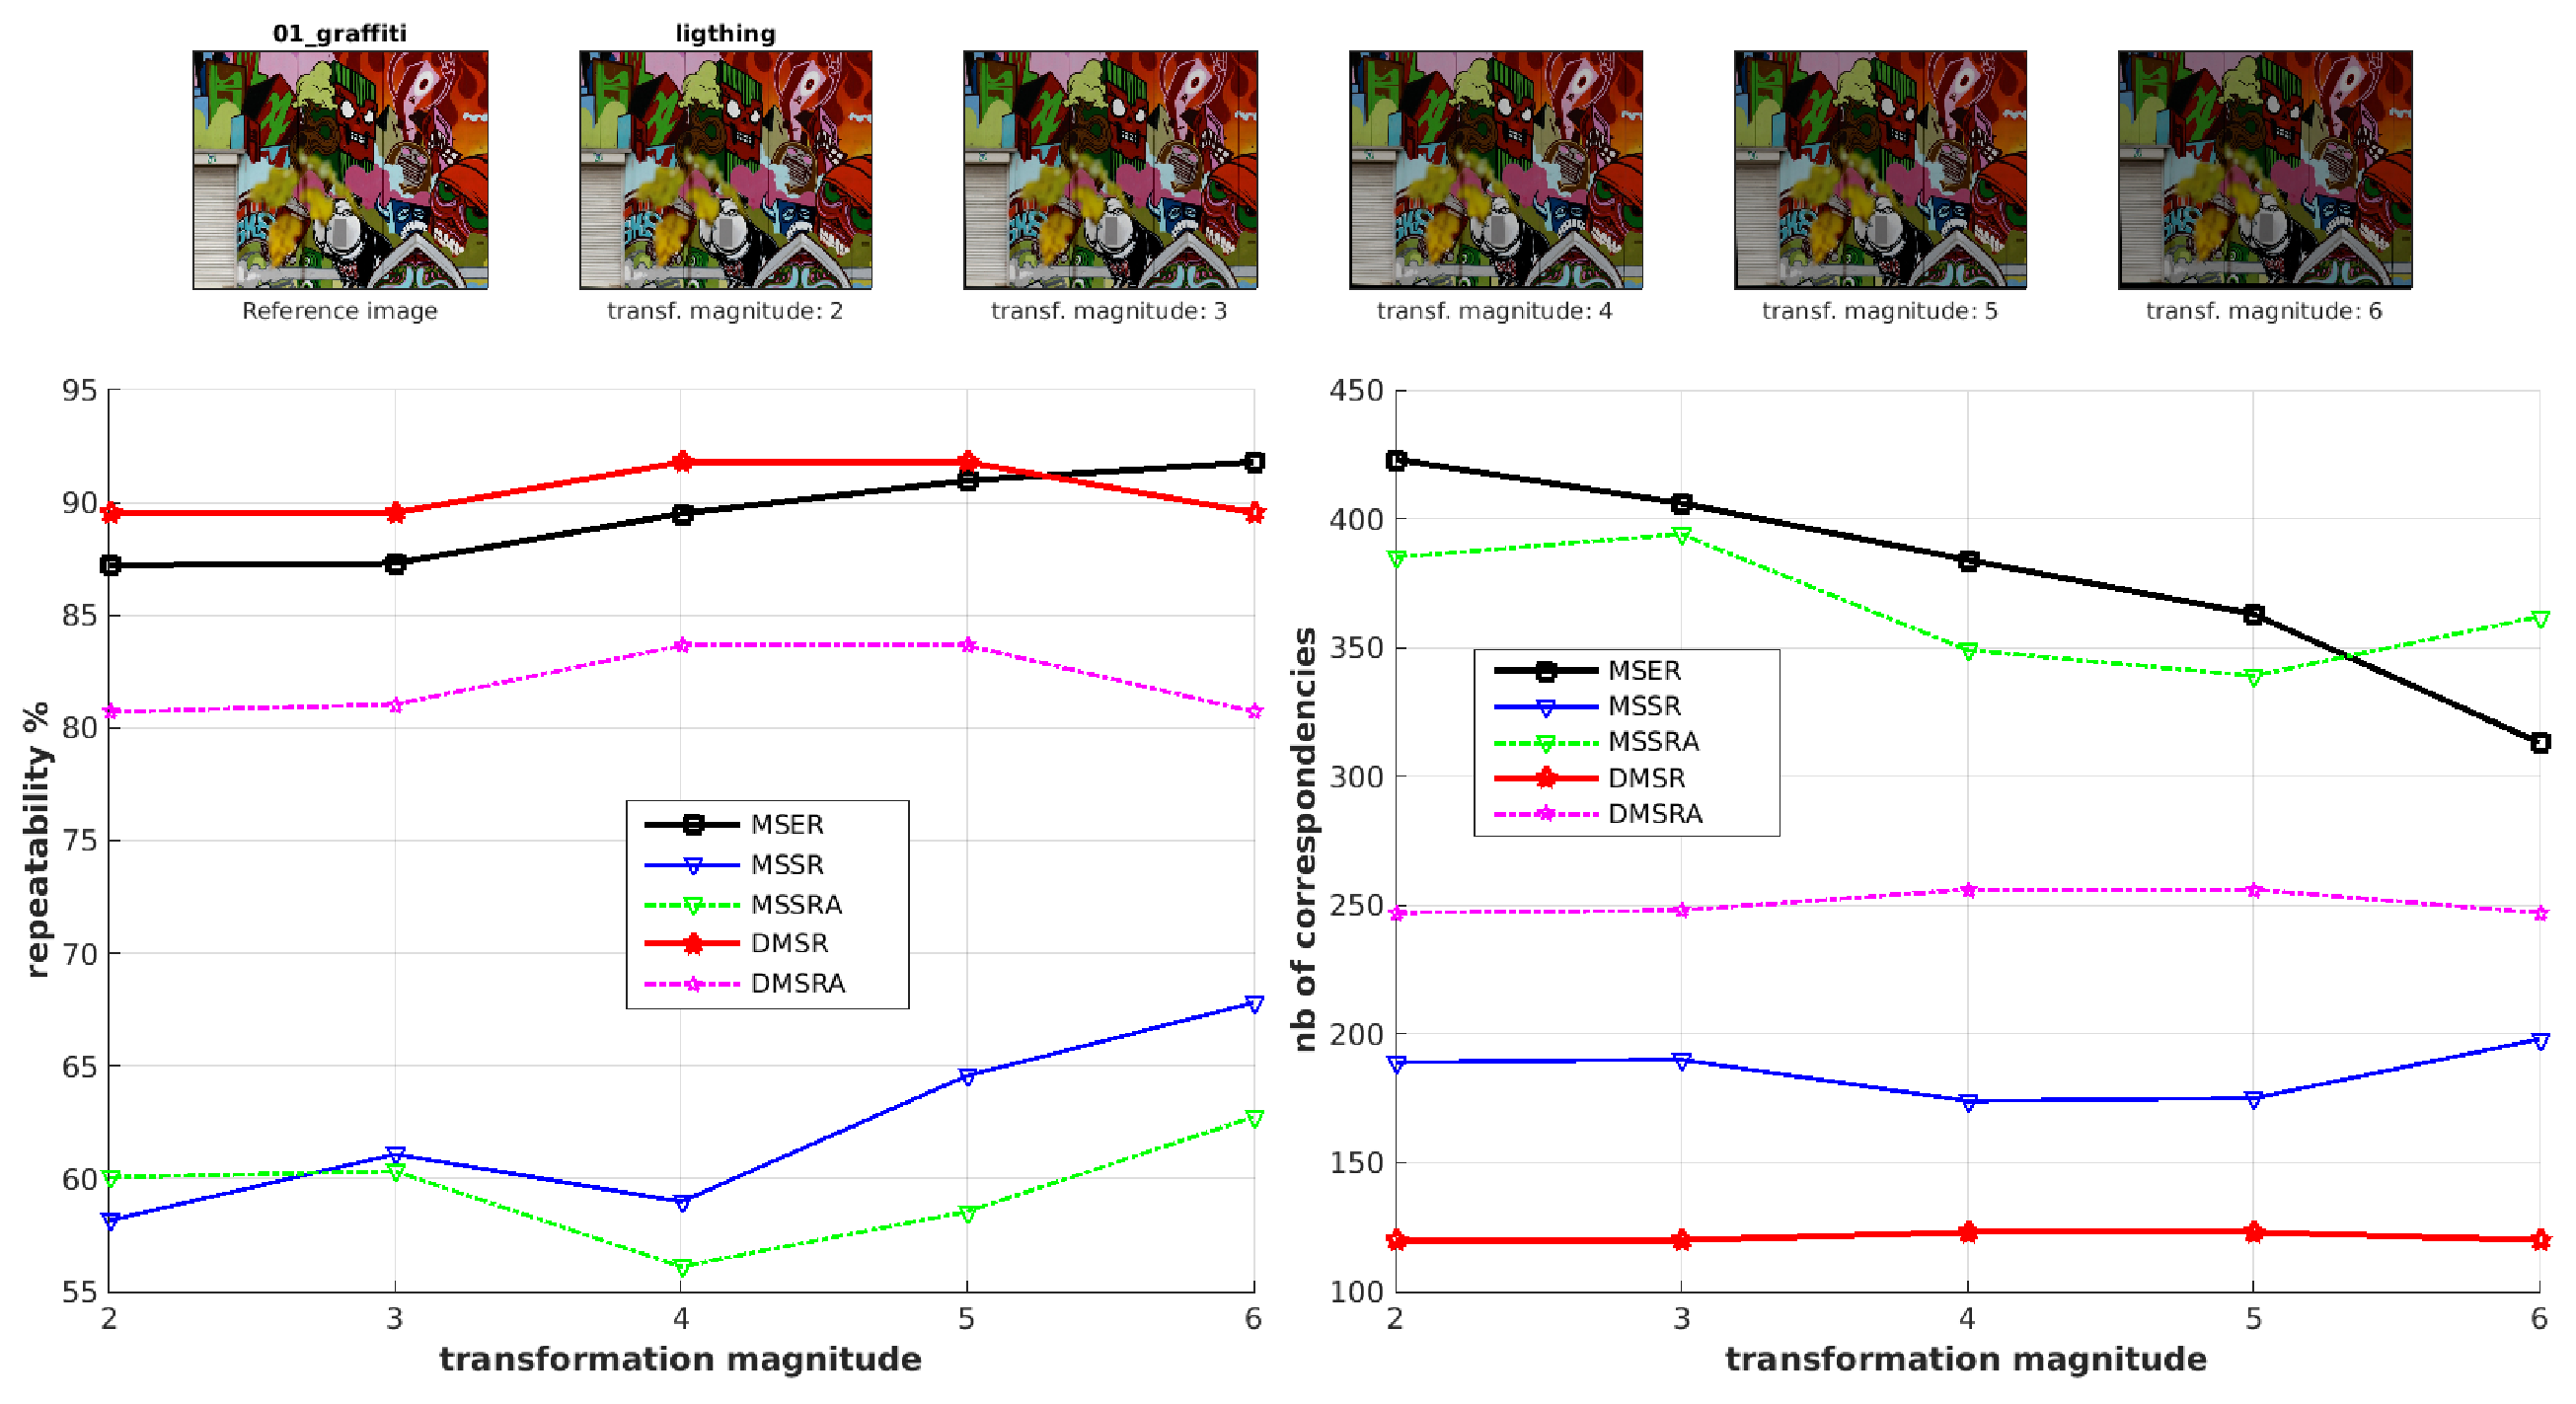
\includegraphics[width=8.4cm]{./Figs/repeatability_all_combined_01_graffiti_ligthing_good}}
 % \vspace{0.2cm}
 % \centerline{(a) MSER}\medskip
\end{minipage}
\hfill
%\vspace{-0.25cm}
\caption{Region detectors on '01\_graffiti', OxFrei dataset.}
\label{fig:det_frei}
%
\end{figure}
%------------------------------------------------------------------------

\begin{figure}[htb]

\begin{minipage}[b]{.9\linewidth}
  \centering
  \centerline{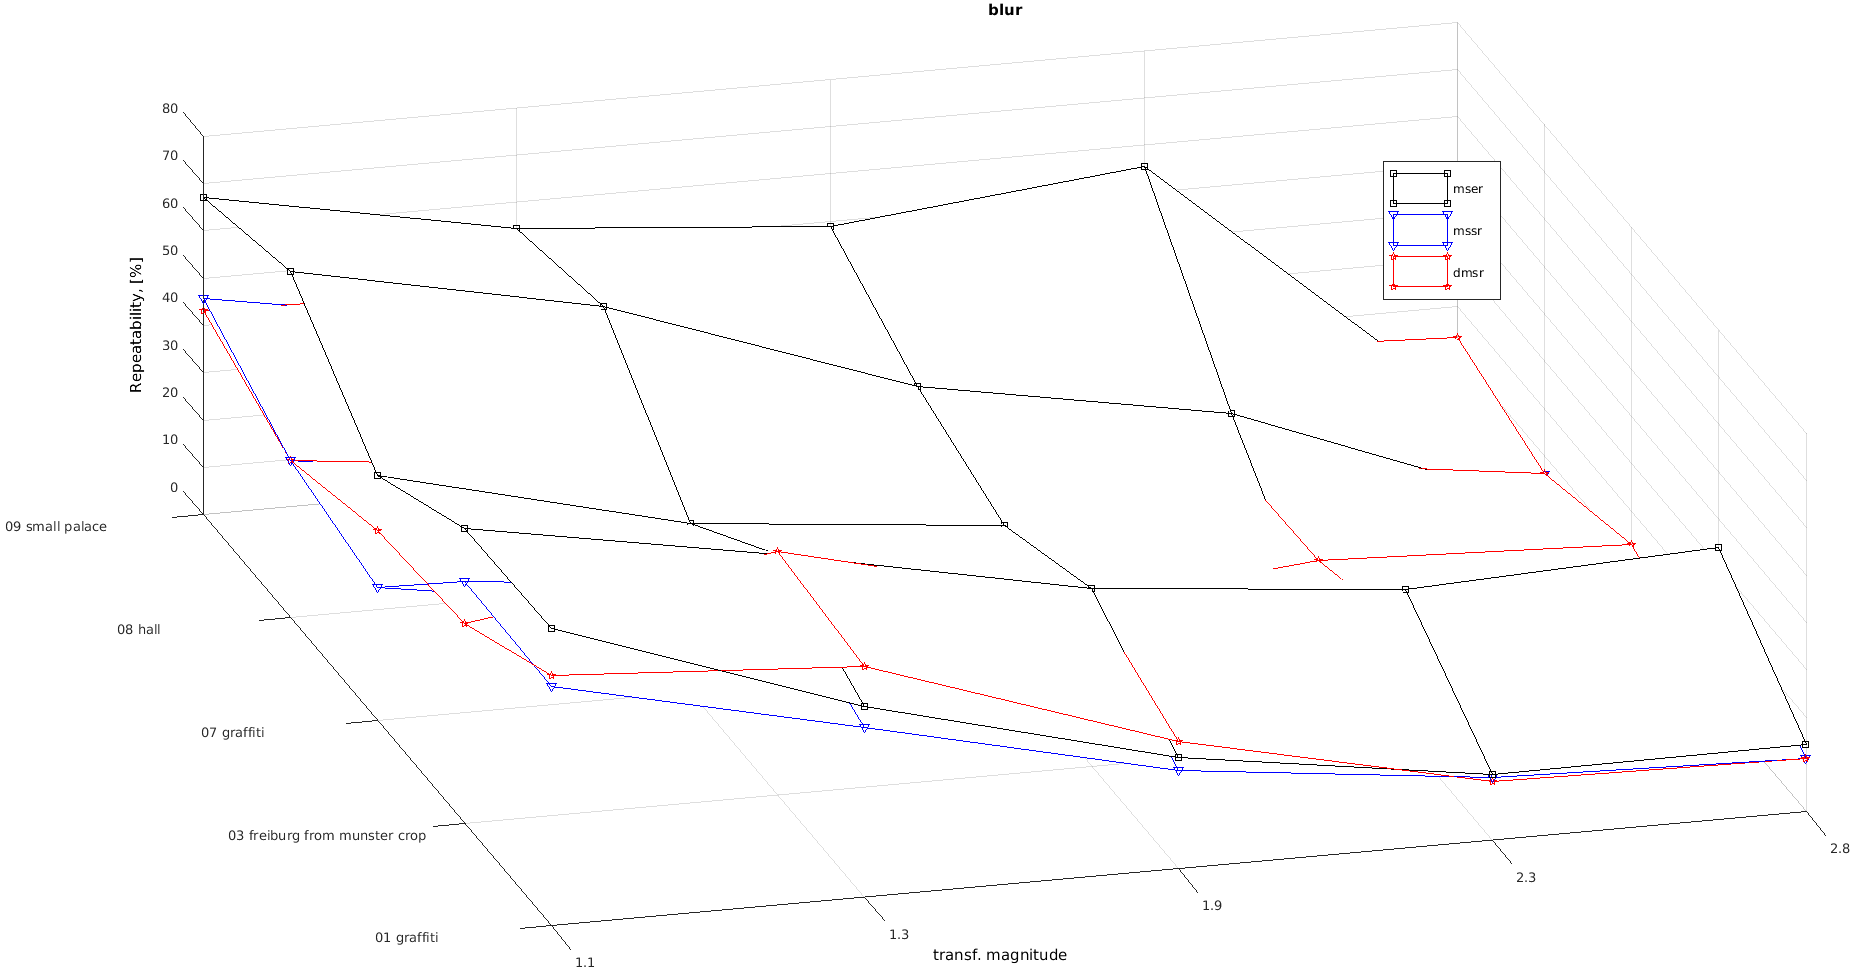
\includegraphics[width=8.4cm]{./Figs/blur_some_combined}}
 % \vspace{0.2cm}
 % \centerline{(a) MSER}\medskip
\end{minipage}
\hfill
%\vspace{-0.25cm}
\caption{Robustness of region detectors to blur.}
\label{fig:blur}
%
\end{figure}
%------------------------------------------------------------------------
%------------------------------------------------------------------------
\subsection{Oxford dataset}
\label{ssec:oxford}
Each image sequence of the Oxford dataset consists of a $1$ base and $5$ increasingly distorted images, \cite{Mikolajczyk:2005}. They are obtained independently of each other and the homographies between each pair $(\I_B,\I_T)$ are the provided  ground truth. Each sequence can be used to test only $1$ transformation $T$.
 %The following sequences have been used: 'Boat'-scale (rotation and zoom), 'Bikes'- blur (Fig. \ref{fig:det_bikes}), 'Graffiti'-viewpoint (Fig. \ref{fig:det_graffiti}), 'Leuven'- lighting (Fig. \ref{fig:leuven_bin}).
For the viewpoint ('graffiti'), best $R$ is achieved by DMSR with up to $72 \%$, which is $10\%$ more than the second performing MSER for $40\deg$ change. DMSR is performing less on the scale sequence ('boat'),but as good or better than MSER on the blur ('bikes', fig. \ref{fig:det_bikes}) and ligthing data ('Leuven').

\subsection{OxFrei dataset}
\label{ssec:combined}
The creators of the Freiburg dataset separated $T$ from image content by applying few artificial $T$ to different base images, \cite{FischerDB14}. Evaluating on the Freiburg dataset proved difficult due to the lack of full transformation parameters documentation. 

To address the shortage of public dataset, the 'OxFrei', combining the strong features of the Oxford and Freiburg datasets, is released, \cite{Rang:dataset}. The Freiburg base images are transformed with all the realistic homographies of the Oxford dataset. In this way, $9$ structured scenes have been created, each subject to $4$ $T$ (blur, lighting, scaling and viewpoint).

To study the robustness, the detectors are compared on all data subject to the same transformation. Figures \ref{fig:det_frei} and \ref{fig:blur} show $R$ under lighting for $1$ and blur for few image sequences. The standart plots (like on Fig. \ref{fig:det_frei}) arecross-sectionsalong the data dimension of the 3D plots (like on Fig. \ref{fig:blur}). The conclusions after examining all 'OxFrei' 3D plots are: MSER is better for zoom and viewpoint (the latter contradicting the limited Oxford data result); DMSR is comparable and better for ligthing and blur  (Fig. \ref{fig:blur}).

{\em More room for some text here...}
\subsection{TNT hi-res benchmark}
\label{ssec:tnt}

The $R$ score of all detectors from \cite{Mikolajczyk:2005} drops down on hi-res images, \cite{CorRos2013}. On the 'underground' sequence from the TNT set, MSER loses up to $25\%$ from $1.5M$ ($R_1$) to $8M$ ($R_4$) resolution. On the contrary, DMSR increases the $R$ score with the resolution increase on 'underground' and 'posters' sequences with up to ..... from $R_1$ to $R_4$, Figure \ref{fig:tnt}. 

\begin{figure}[htb]

\begin{minipage}[b]{.9\linewidth}
  \centering
  \centerline{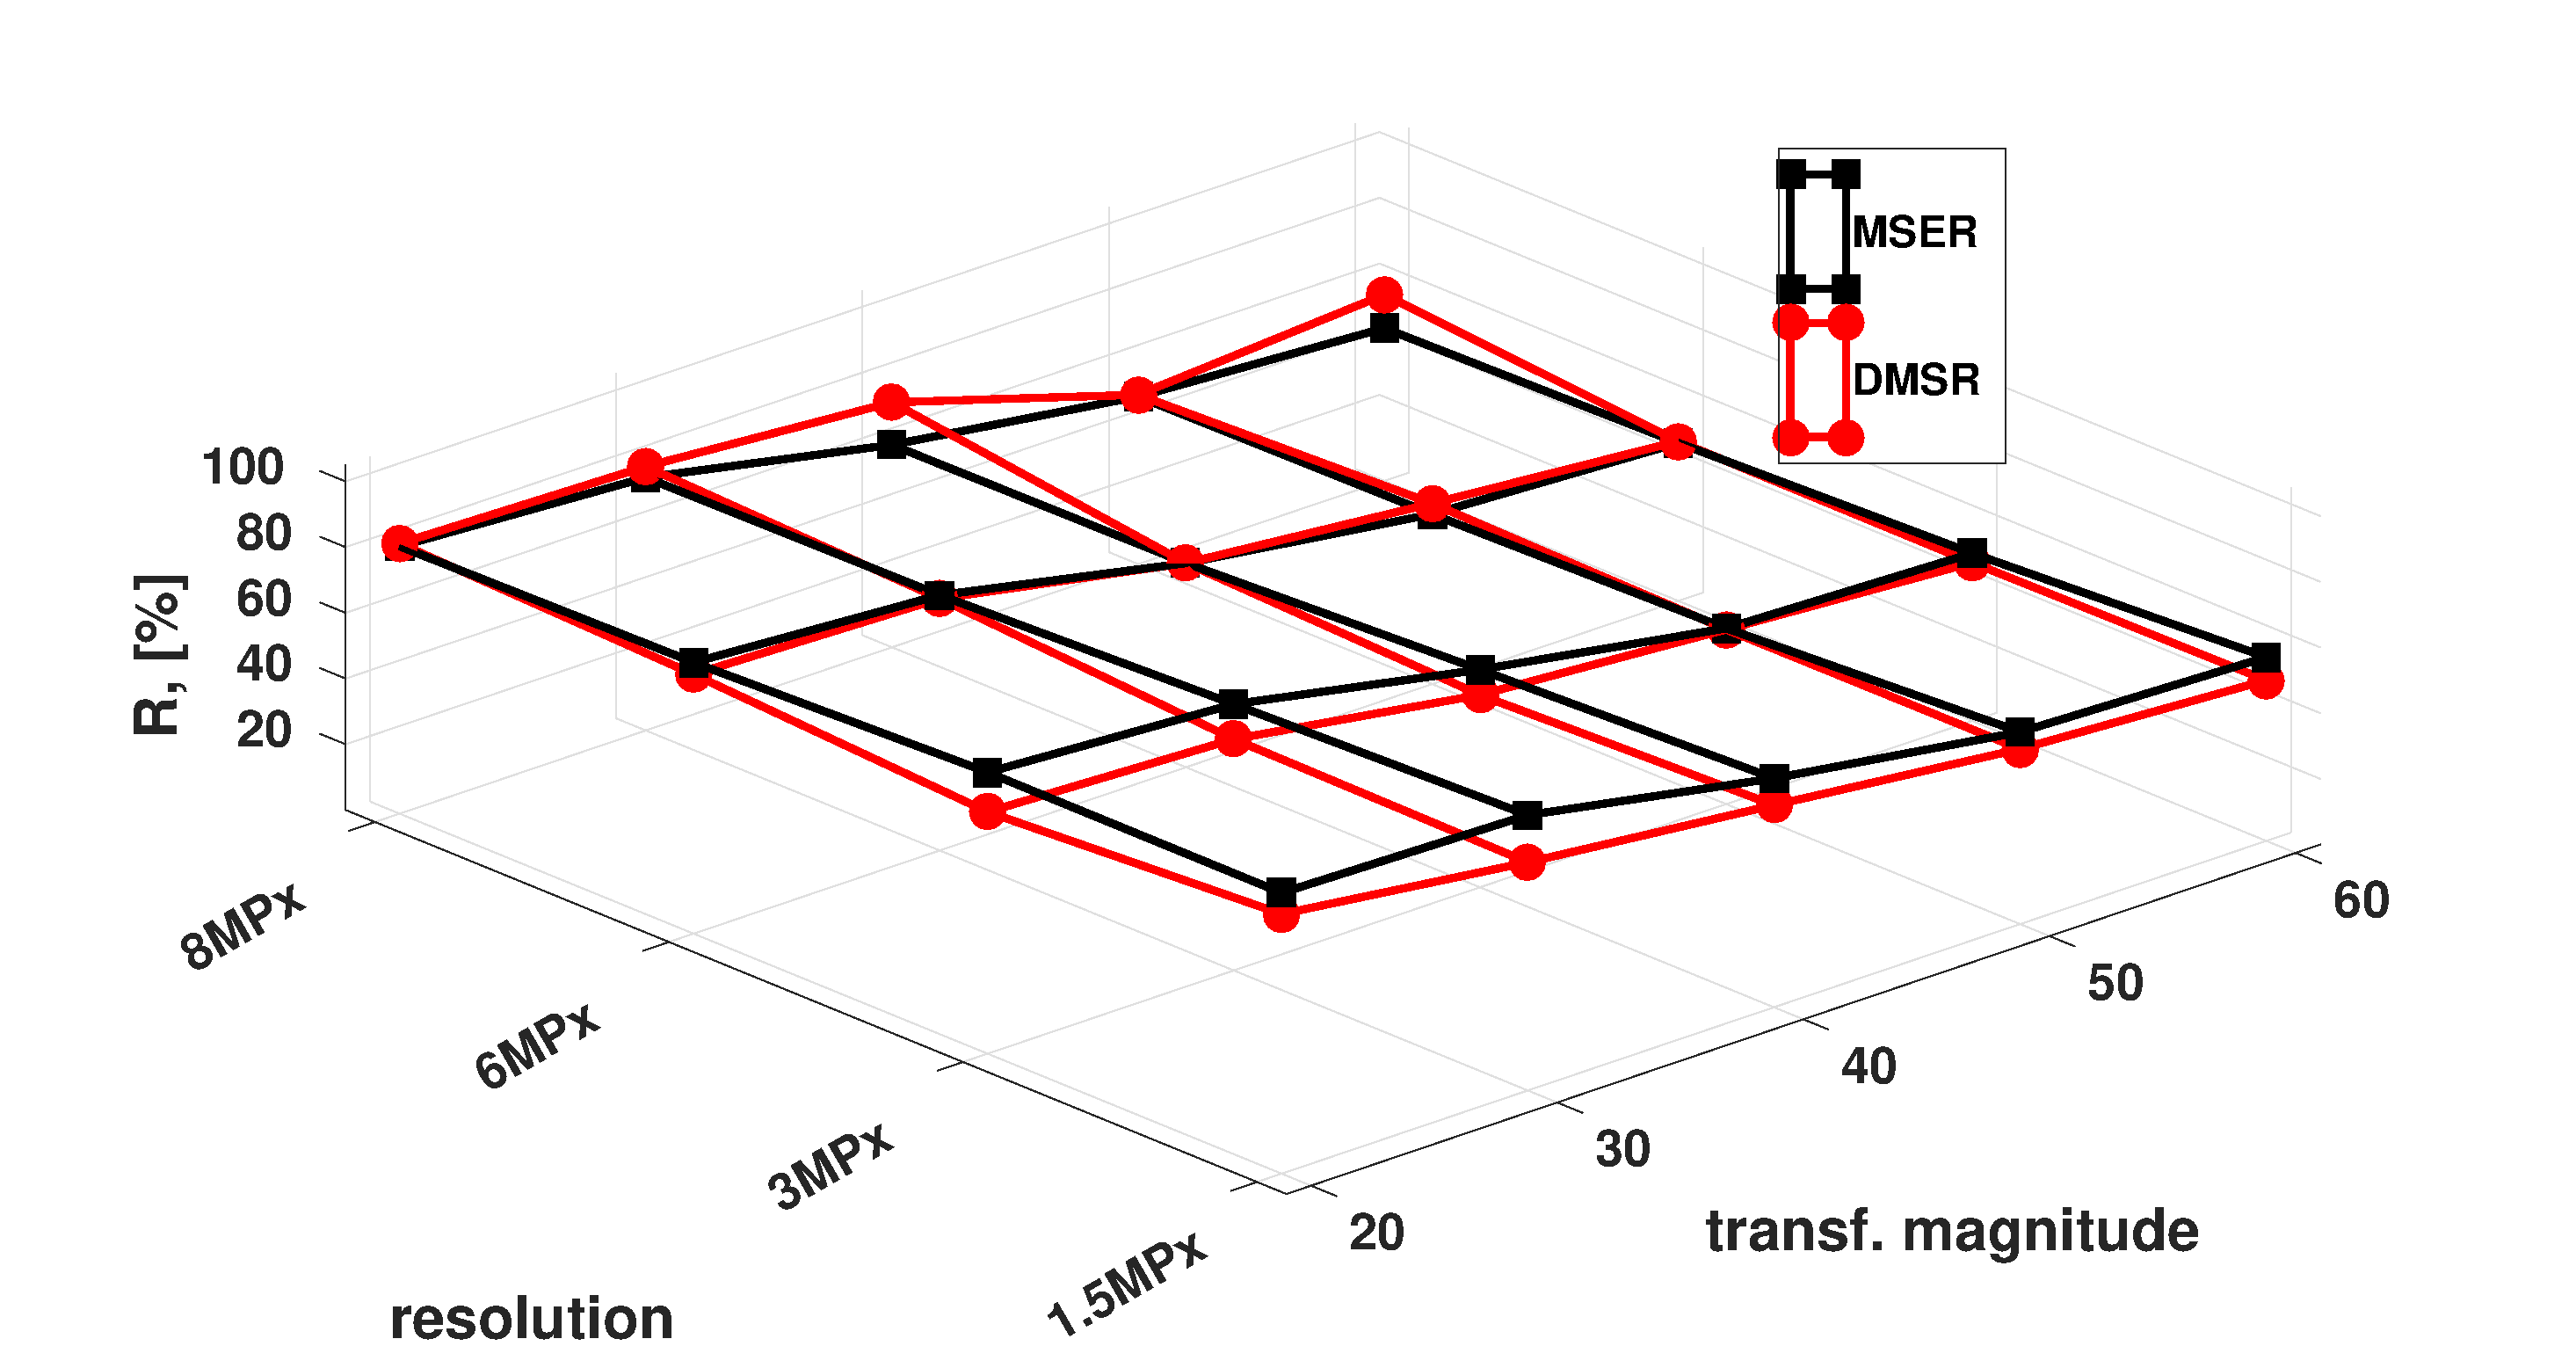
\includegraphics[width=8.4cm]{./Figs/posters_rep}}
 % \vspace{0.2cm}
 % \centerline{(a) MSER}\medskip
\end{minipage}
\hfill
\caption{Robustness of region detectors to image resolution and viewpoint.}
\label{fig:tnt}
%
\end{figure}
%------------------------------------------------------------------------
\begin{figure}[htb]

\begin{minipage}[b]{0.9\linewidth}
  \centering
  \centerline{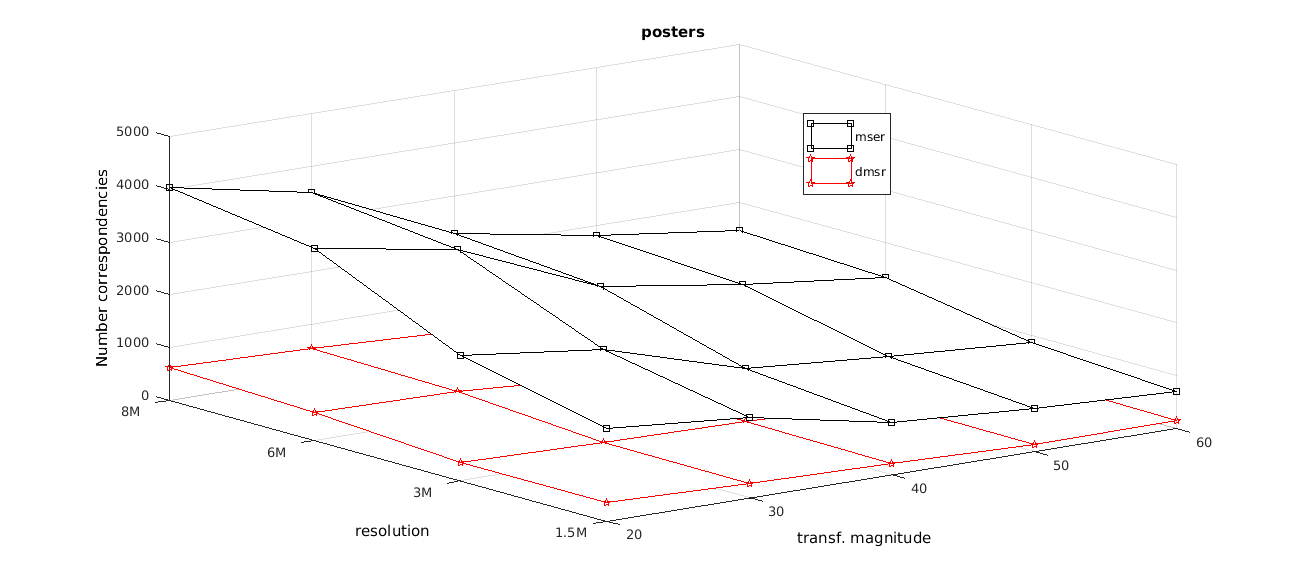
\includegraphics[width=8.4cm]{./Figs/posters_numreg}}
 % \vspace{0.2cm}
 % \centerline{(b) DMSR}\medskip
\end{minipage}
%\vspace{-0.25cm}
\caption{Number of regions with increase of image resolution under viewpoint transformation.}
\label{fig:tnt_numreg}
%
\end{figure}
%------------------------------------------------------------------------

As an efficiency and stability indicators, the $N_C$ plane of DMSR is at the lowest values with the least slope among all detectors (e.g. sections on Fig. \ref{fig:det_bikes} and \ref{fig:det_bikes}, right and the plane on Fig. \ref{fig:tnt_numreg}). Using all $4$ types of  regions generally does not improve performance over using only $ISS$ (holes and islands).

\subsection{Animal and plant biometrics}
\label{ssec:bio}
The DMSR detector has been compared to MSER on several small animal individual photo-ID datasets (humpback whales, leatherback turtles, newts) and on a wood species identification dataset. In all cases DMSR produces less and perceptually more acurate salient regions, figures \ref{fig:tails}, \ref{fig:turtle} and \ref{fig:wood}. For the wood microscopy images, it is important to measure the geometric properties of the cells, which is achievable with the DMSR regions, unlike the very large number of non-precise and overlapping MSER regions.

\section{CONCLUSIONS}
Combining data-driven binarization and binary morphological operations leads to salient region detector, DMSR, with comparable to superior performance to MSER. It produces much smaller number of regions, a very desired property in the large scale data processing. DMSR copes better with blur, lighting and increased resolution.  For detection bench-marking, high-resolution and transformation independent datasets should become the standard. DMSR gives perceptually salient regions, which makes it a good choice for scientific imagery analytic tasks.  
\label{sec:concl}




% To start a new column (but not a new page) and help balance the last-page
% column length use \vfill\pagebreak.
% -------------------------------------------------------------------------
%\vfill
%\pagebreak


%\section{REFERENCES}
%\label{sec:ref}


% References should be produced using the bibtex program from suitable
% BiBTeX files (here: strings, refs, manuals). The IEEEbib.bst bibliography
% style file from IEEE produces unsorted bibliography list.
% -------------------------------------------------------------------------
\bibliographystyle{IEEEbib}
\bibliography{icip2016}

\end{document}
